% This must be in the first 5 lines to tell arXiv to use pdfLaTeX, which is strongly recommended.
\pdfoutput=1
% In particular, the hyperref package requires pdfLaTeX in order to break URLs across lines.

\documentclass[11pt]{article}

%----------------------------------------
% Custom packages
%----------------------------------------
% Used in equations
\usepackage{amsmath}

% Figures
\usepackage{subfig}
\usepackage{graphicx}

%----------------------------------------

% Remove the "review" option to generate the final version.
\usepackage[review]{acl}

% Standard package includes
\usepackage{times}
\usepackage{latexsym}

% For proper rendering and hyphenation of words containing Latin characters (including in bib files)
\usepackage[T1]{fontenc}
% For Vietnamese characters
% \usepackage[T5]{fontenc}
% See https://www.latex-project.org/help/documentation/encguide.pdf for other character sets

\usepackage[utf8]{inputenc}

% This is not strictly necessary, and may be commented out,
% but it will improve the layout of the manuscript,
% and will typically save some space.
\usepackage{microtype}

% If the title and author information does not fit in the area allocated, uncomment the following
%
%\setlength\titlebox{<dim>}
%
% and set <dim> to something 5cm or larger.

\title{Contrastive Pre-Training for Text Alignment}

% Author information can be set in various styles:
% For several authors from the same institution:
% \author{Author 1 \and ... \and Author n \\
%         Address line \\ ... \\ Address line}
% if the names do not fit well on one line use
%         Author 1 \\ {\bf Author 2} \\ ... \\ {\bf Author n} \\
% For authors from different institutions:
% \author{Author 1 \\ Address line \\  ... \\ Address line
%         \And  ... \And
%         Author n \\ Address line \\ ... \\ Address line}
% To start a seperate ``row'' of authors use \AND, as in
% \author{Author 1 \\ Address line \\  ... \\ Address line
%         \AND
%         Author 2 \\ Address line \\ ... \\ Address line \And
%         Author 3 \\ Address line \\ ... \\ Address line}

\author{Sebastian Schmidt \and Jonas Probst \and Cecilia Graiff \\
  Leipzig University / Augustusplatz 10, 04109 Leipzig
  }
% \texttt{ss56pupo@studserv.uni-leipzig.de}
% \texttt{gv53ozag@studserv.uni-leipzig.de}
% \texttt{cg67qowo@studserv.uni-leipzig.de}

\begin{document}
\maketitle
\begin{abstract}
Contrastive learning was applied successfully in self-supervised settings for several natural language tasks.
Inspired by the approach of supervised contrastive learning by Khosla et. al \cite{khosla:2020}, we applied a similar approach to pre-train encoders for text alignment, a subtask of text reuse identification.
%Todo: Adapt based on experimental findings
The classifiers that were trained on top of the sentence embeddings of the pre-trained encoders were able to outperform benchmark architectures in which the linear classifier was trained together with the underlying encoder.  
\end{abstract}

\section{Introduction}
\label{sec:intro}
Text reuse identification has been approached in various manual and automated ways \cite{gienapp:2021, potthast:2013e}. 
The goal of the research presented in this paper was to evaluate the performance of contrastive pre-training, which was successfully applied to computer vision \cite{khosla:2020}, on the subtask of text alignment.\\
Towards that goal, a pre-trained sentence transformer was fine-tuned in two separate ways.
First, the contrastive model was trained in a two-step fashion. 
(1) Pre-train the transformer using different contrastive learning objectives, and (2) freeze the weights of the transformer and fit a classifier on top of the embeddings.
Afterwards, a supervised benchmark was created by adding a classifier on top of the sentence embeddings created by the encoder and fitting the weights of both the classifier as well the transformer on a training set of sentence pairs.
In order to evaluate the effect of contrastive pre-training, both types of fine-tuned models were applied to a set of evaluation datasets used for text reuse identification. 



\section{Related work}
\label{sec:relWork}
The research presented in this paper draws from two main fields: Text reuse identification and contrastive learning.
Therefore, this section gives and overview on related work from both areas.

\subsection{Text alignment}
The task of text reuse identification is split into two subtasks. 
While source retrieval is concerned with the search for candidate documents from which a suspicious document may have reused material, text alignment deals with the identification of specific passages that were taken from these candidates \cite{potthast:2013e}.\\
Given that research on text alignment has a long history, a broad range of approaches has been applied to the task: %Todo: Brief summary of previous work (Potthast Paper)
Because of the advances that transformer-based architectures have made in all areas of natural language processing, it is to be expected that these models also achieve considerable performance on text alignment. %Todo: Check work on text alignment (or simply paraphrasing); Hamlet paper: Do NN help?
The question to be answered in the research at hand is how contrastive pre-training influences the performance of transformer-based models in this task.
%Todos
% - Mention evaluation competition and benchmark datasets


\subsection{Contrastive learning}
\label{sec:contrLearn}
The majority of classification tasks in machine learning is approached in a supervised fashion.
Generally, the model is trained to assign data points to a set of pre-defined classes like digits or different kinds of objects, animals, etc. %todo: quote MNIST and ImageNet
While this approach is very successful on a broad range of tasks, it has certain limitations.
Specifically, supervised learning cannot be applied to problems in which the number of classes is unknown at the moment of training. \\
In order to address this gap, Chopra et al. \cite{chopra:2005} developed the idea of contrastive learning.
The main idea is to train the model not on the task assigning data points to predefined classes but on identifying if two data points belong to the same class.
Chopra et al. \cite{chopra:2005} coined the term energy function $d(x_1, x_2)$ and illustrated it using the task of facial recognition:
The value of $d$ should be low for images of two faces $x_1$ and $x_2$ from the same person and high for image pairs belonging to different people.
Ultimately, the goal of contrastive learning is to train the embedding space of the model so that the distance of data points in that space reflects their semantic similarity in the input space.
In the context of this paper, this means that the embeddings created by the sentence transformer should have a low distance for pairs of paraphrases and a high distance otherwise.

\subsubsection{Contrastive pre-training}
Due to the design of its loss functions, contrastive learning is well suited to pre-train models so that the generated embeddings reflect semantic information about the corresponding input.
As as consequence, it has been applied in a self-supervised settings for problems in natural language processing \cite{mikolov:2013, yang:2015, devlin:2018}.\\
The self-supervised application, however, comes with a certain risk as pointed out by Khosla et al.:
Because the training is conducted on data without explicit labels, there is no guarantee that the negative samples come from a different distribution than the anchor sample \cite{khosla:2020}.
In their paper, the authors showed that contrastive pre-training on labeled not only avoids this risk but leads to improved performance on downstream tasks.
Specifically, the classifier that was trained on the embeddings of the pre-trained image encoder was able to improve Top-1 accuracy on ImageNet by roughly one percent over benchmark models like AutoAugment, RandAugment, and CutMix \cite{cubuk:2018, cubuk:2019, yun:2019}.\\
Inspired by these results, we evaluated the effect of supervised contrastive pre-training on paraphrase detection.

\subsubsection{Contrastive losses}
In order to evaluate multiple different forms of contrastive learning, the encoder was pre-trained using three different loss functions.\\
The first function, pairwise loss, was proposed by Chopra et al. to learn a similarity metric in settings where not all possible classes are available upfront \cite{chopra:2005}.
As the name suggests, a pair of inputs $x_1$ and $x_2$ (e.g., sentences) is processed by a Siamese architecture of two encoders with identical weights $\theta$ to create the two embeddings $f_\theta(x_1)$ and $f_\theta(x_1)$.\\
Afterwards, the Euclidean distance $d(x_1, x_2)=\| f_\theta(x_1) - f_\theta(x_2) \|_2$ between the two inputs is determined and the loss calculated based on a label $y$.
If the label is one, both inputs belong to the same distribution and the loss is equal to the distance of the embeddings.
Otherwise, the loss is equal to the difference between the distance and a minimum margin $\epsilon$ that two inputs from separate distributions should be apart.
This leads to the following definition of the loss value for one pair:
\begin{equation}\begin{split}
\label{eq:pairLoss}
    \mathcal{L}_\text{P} = y*d(x_1, x_2)^2 \\
        + (1-y)*\max[0, \epsilon - d(x_1, x_2)]^2
\end{split}\end{equation}
The value for the margin was chosen to be $\epsilon=0.5$ based on experiments on the Microsoft Research Paraphrase Corpus (MRPC), that is available in the GLUE benchmark collection \cite{dolan:2005, wang:2018}.  
The development of the distance values in these experiments indicated that higher values increased the risk of overfitting.
A visualization of different margin values can be seen in Figure \ref{fig:dist_dev}.\\
\begin{figure*}[!tbp]
  \centering
  \subfloat[Margin = 0.3]{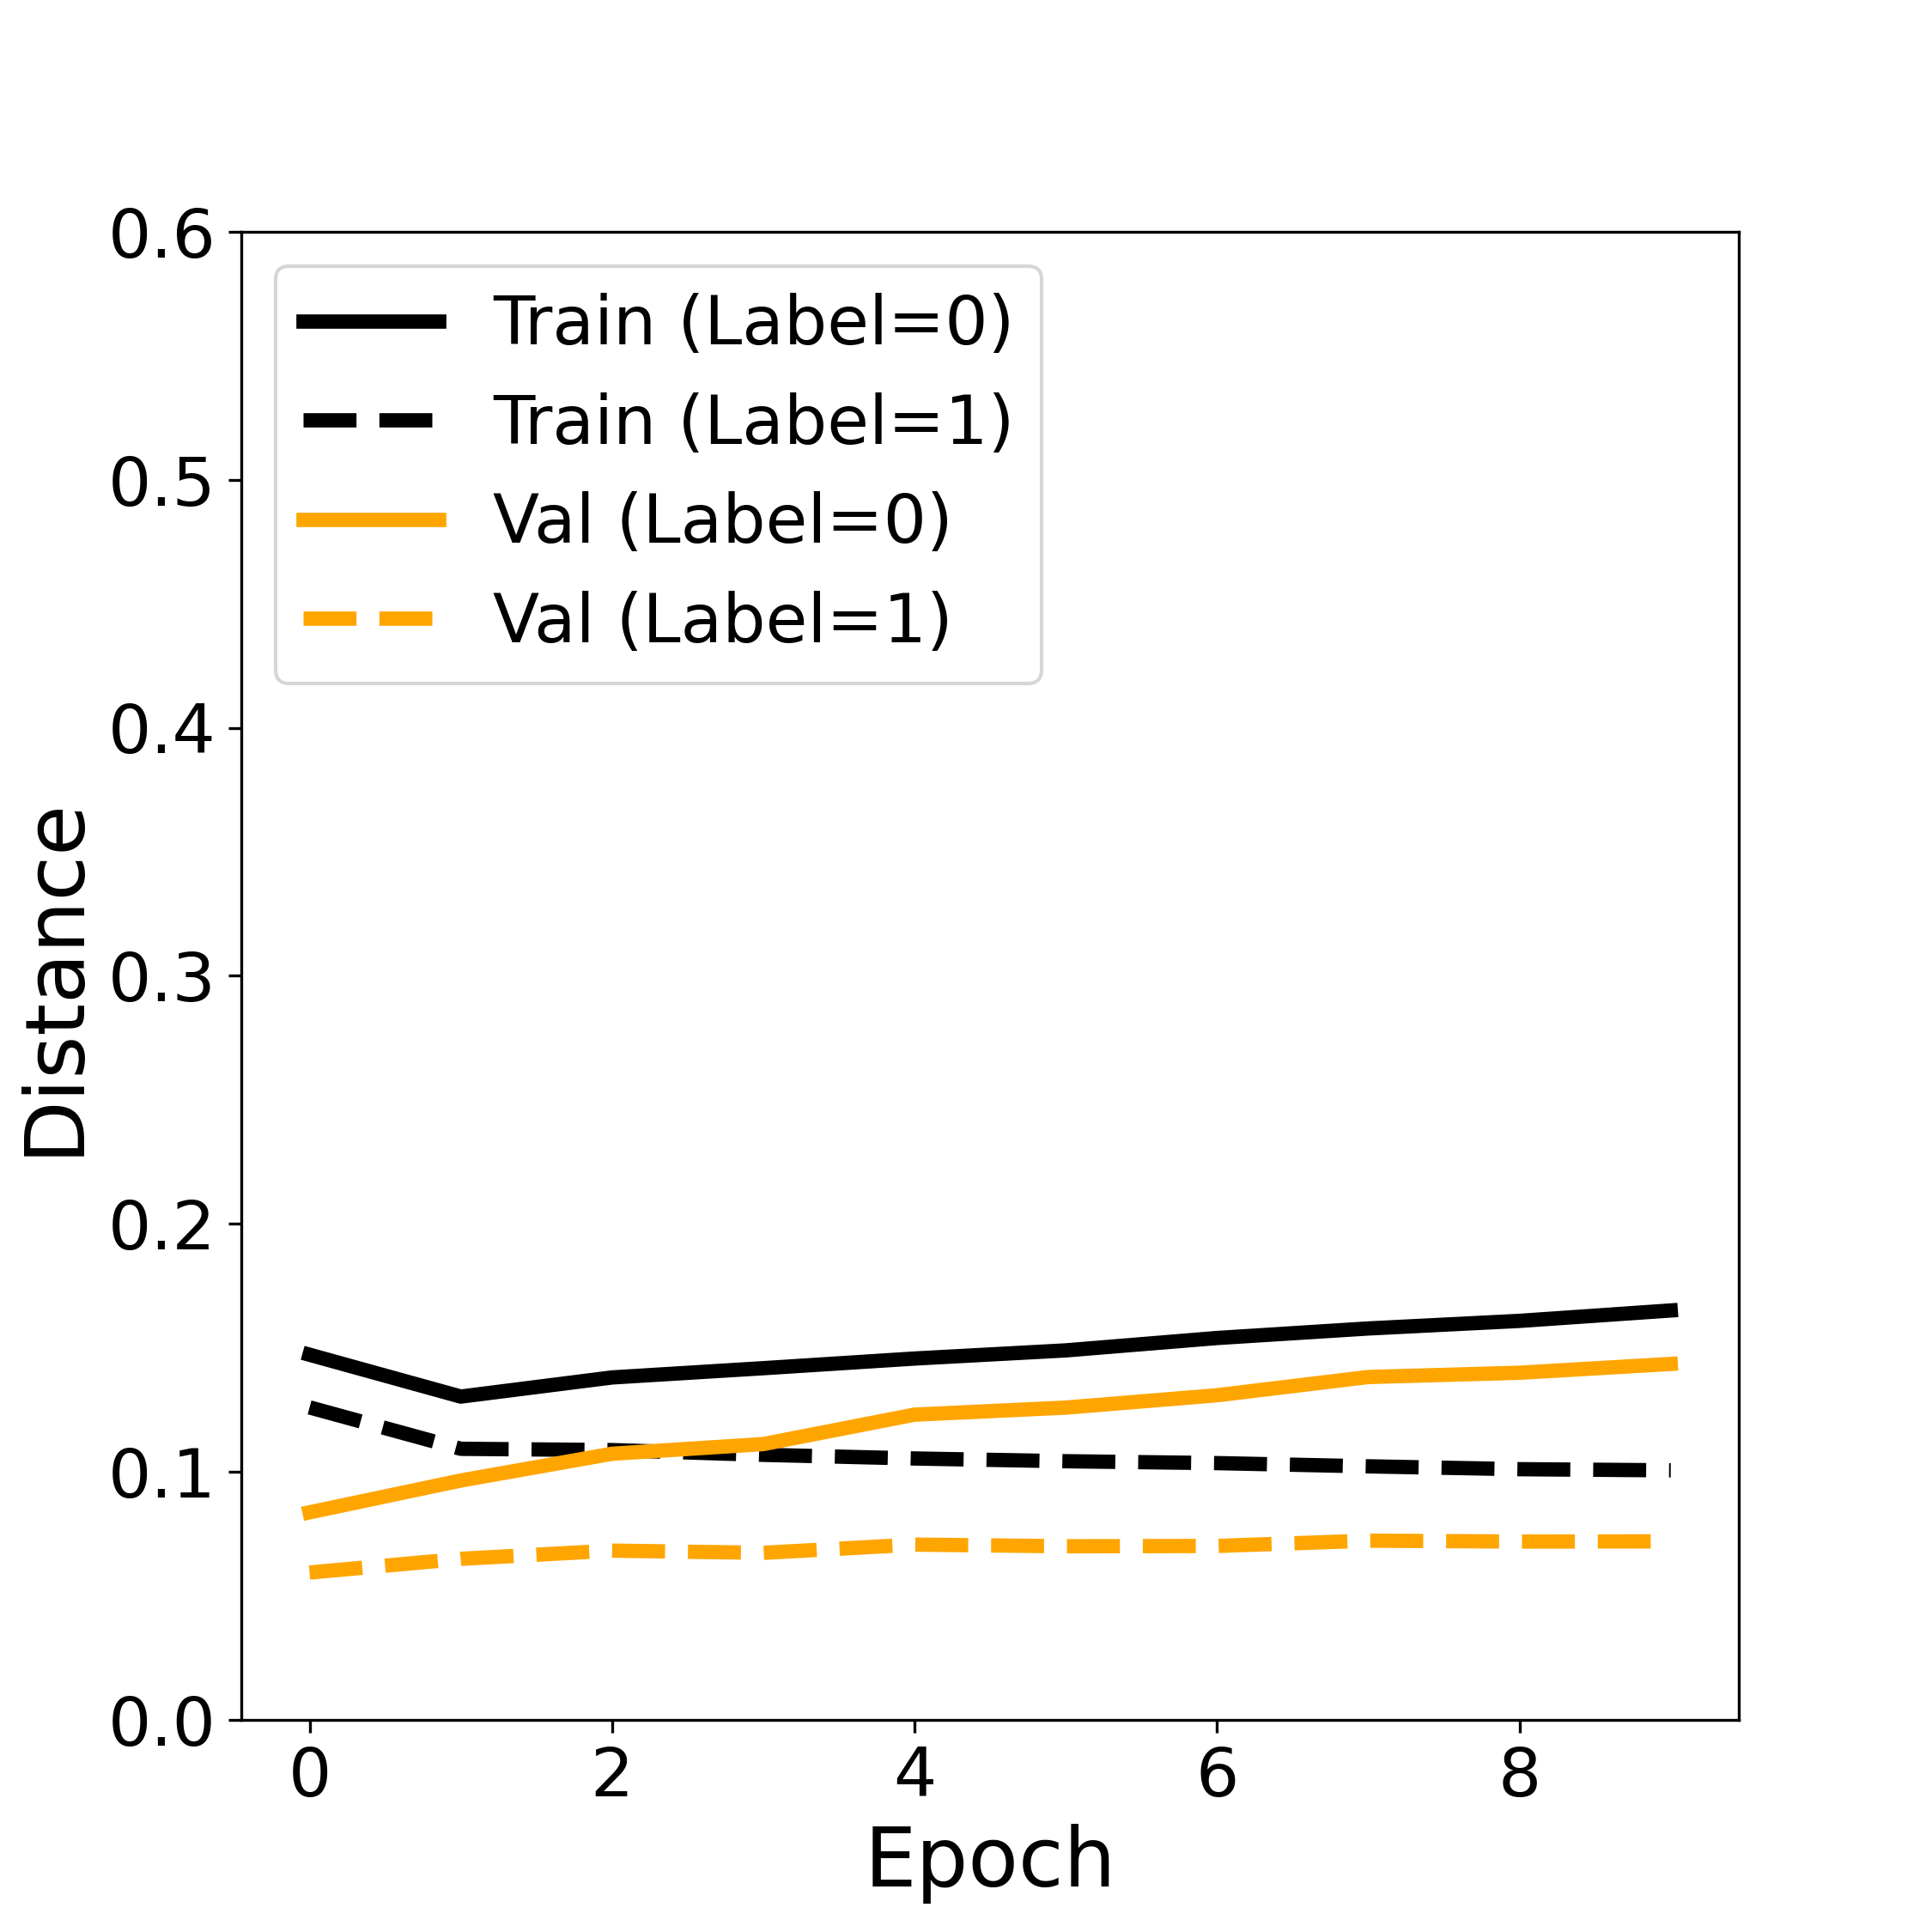
\includegraphics[width=0.33\textwidth]{Images/Distance_eps3.png}\label{fig:eps3}}
  \subfloat[Margin = 0.5]{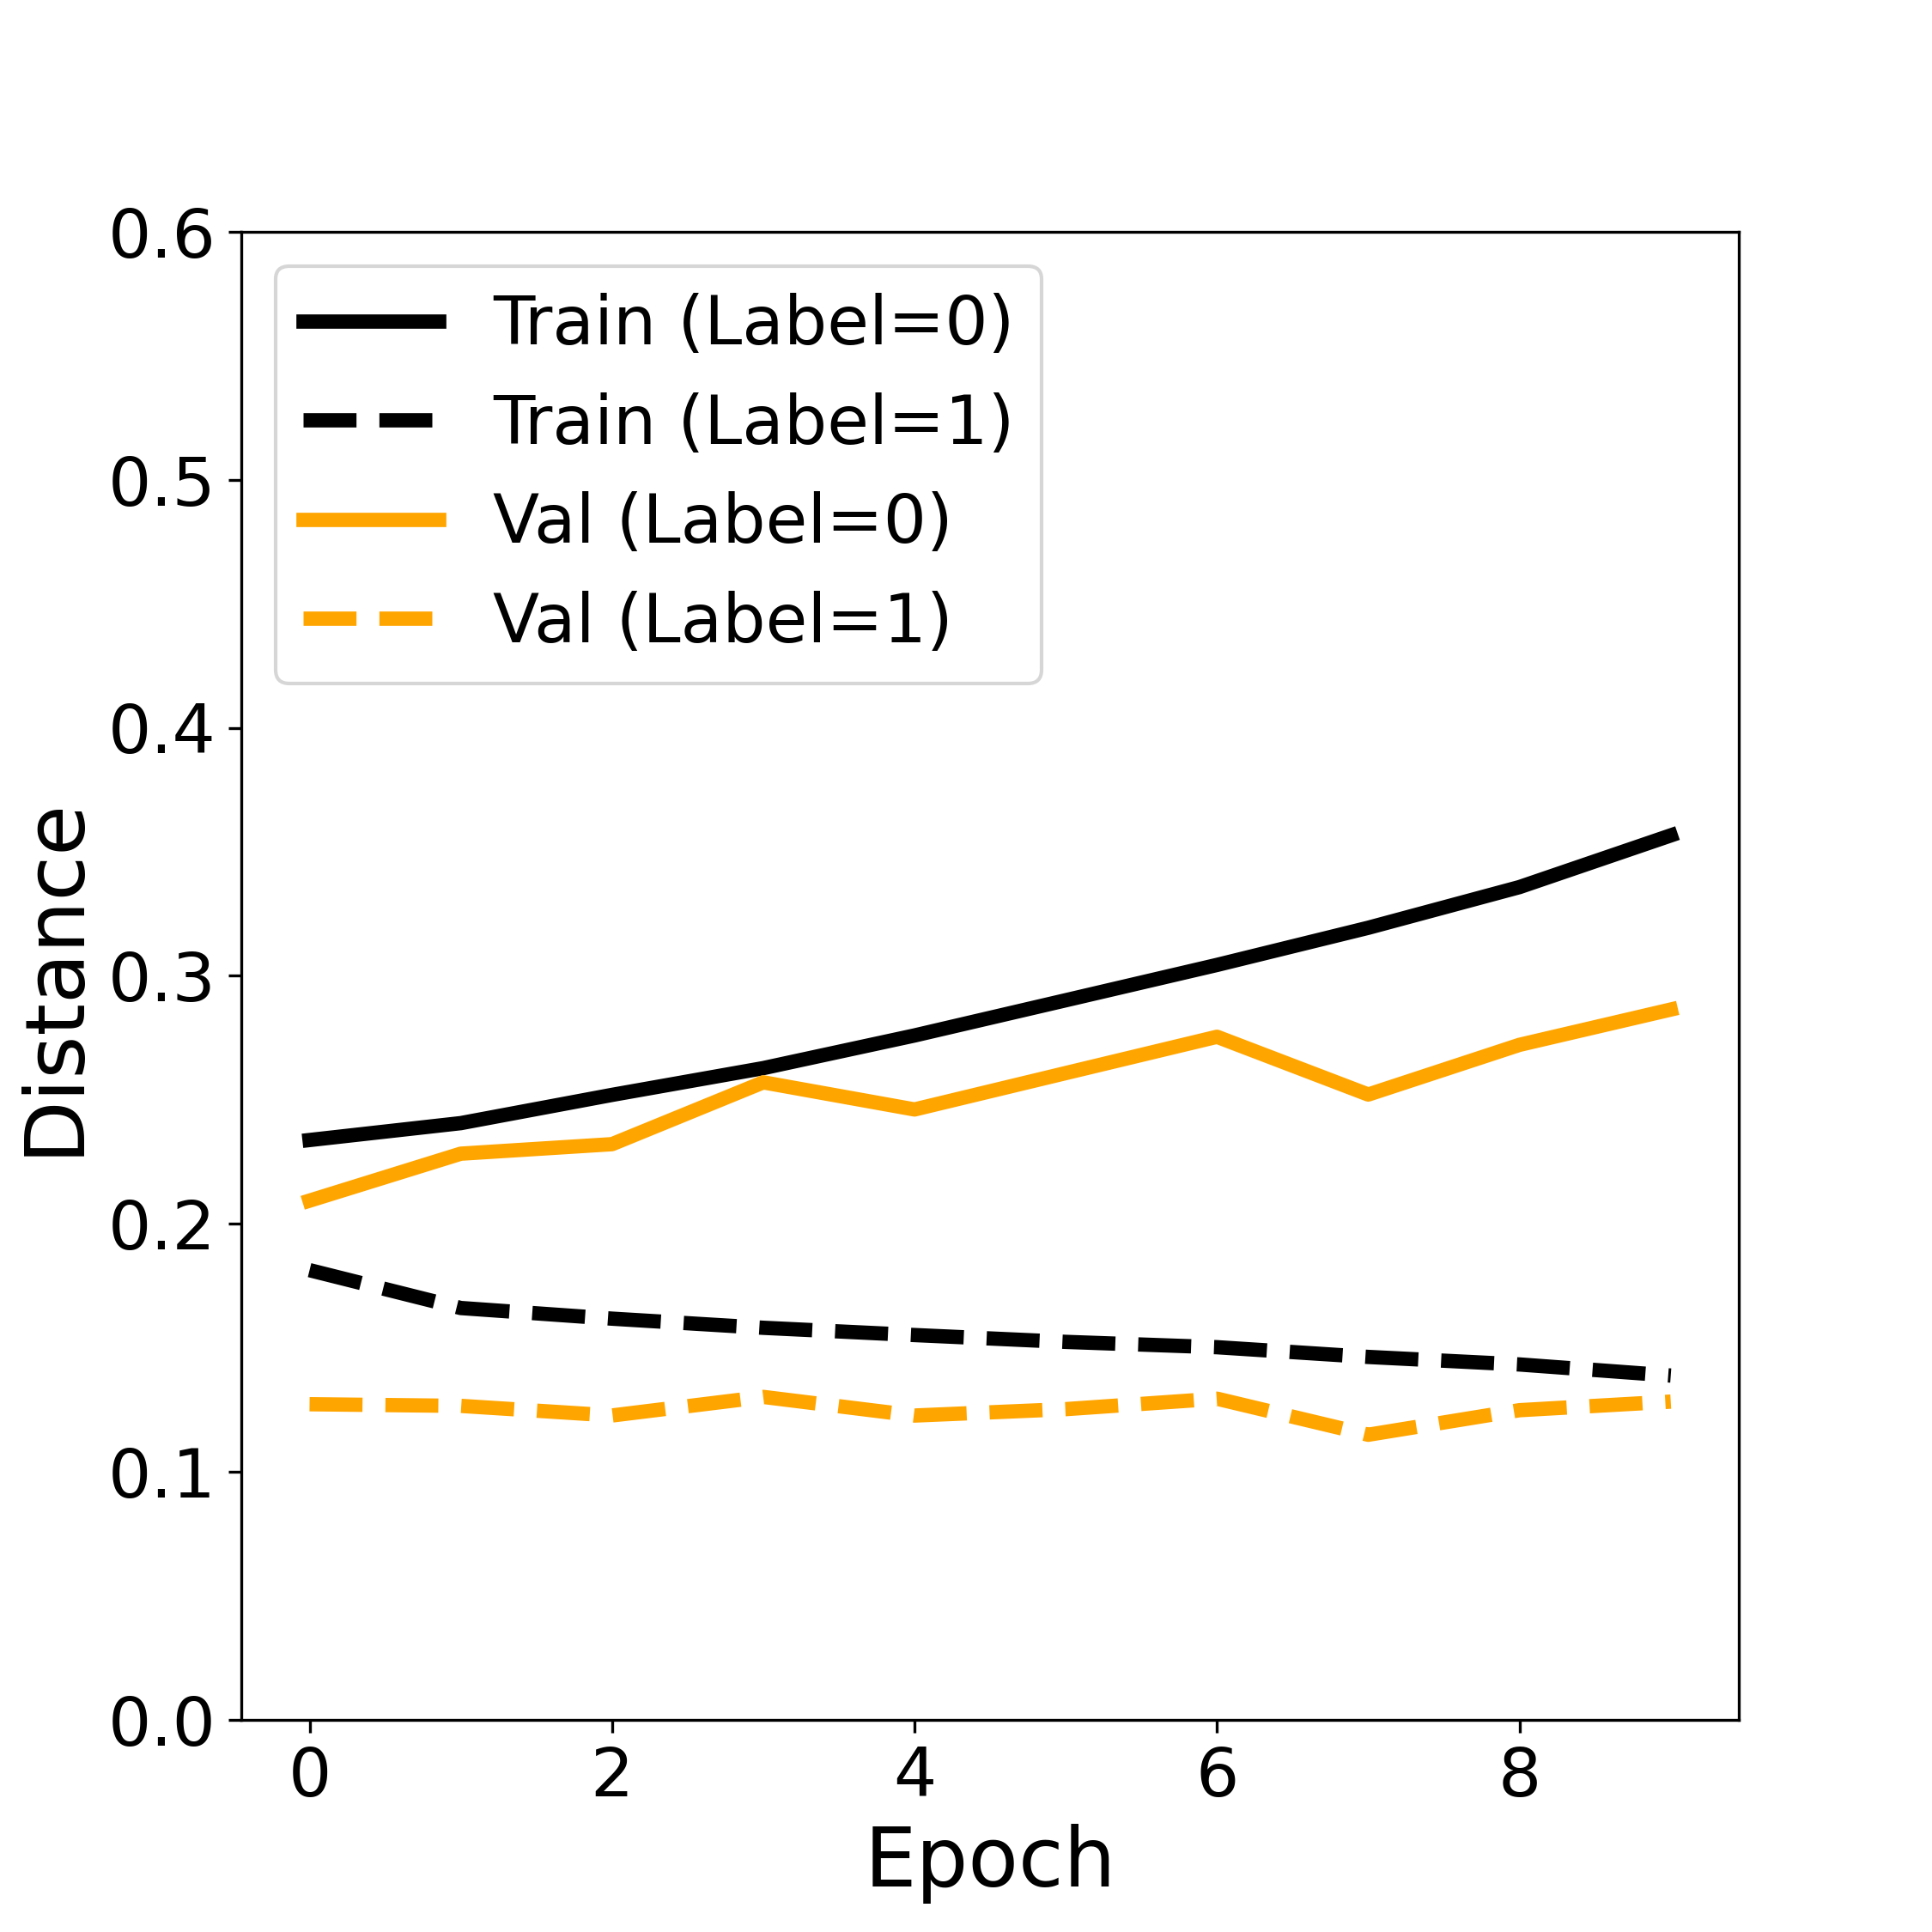
\includegraphics[width=0.33\textwidth]{Images/Distance_eps5.png}\label{fig:eps5}}
  \subfloat[Margin = 0.7]{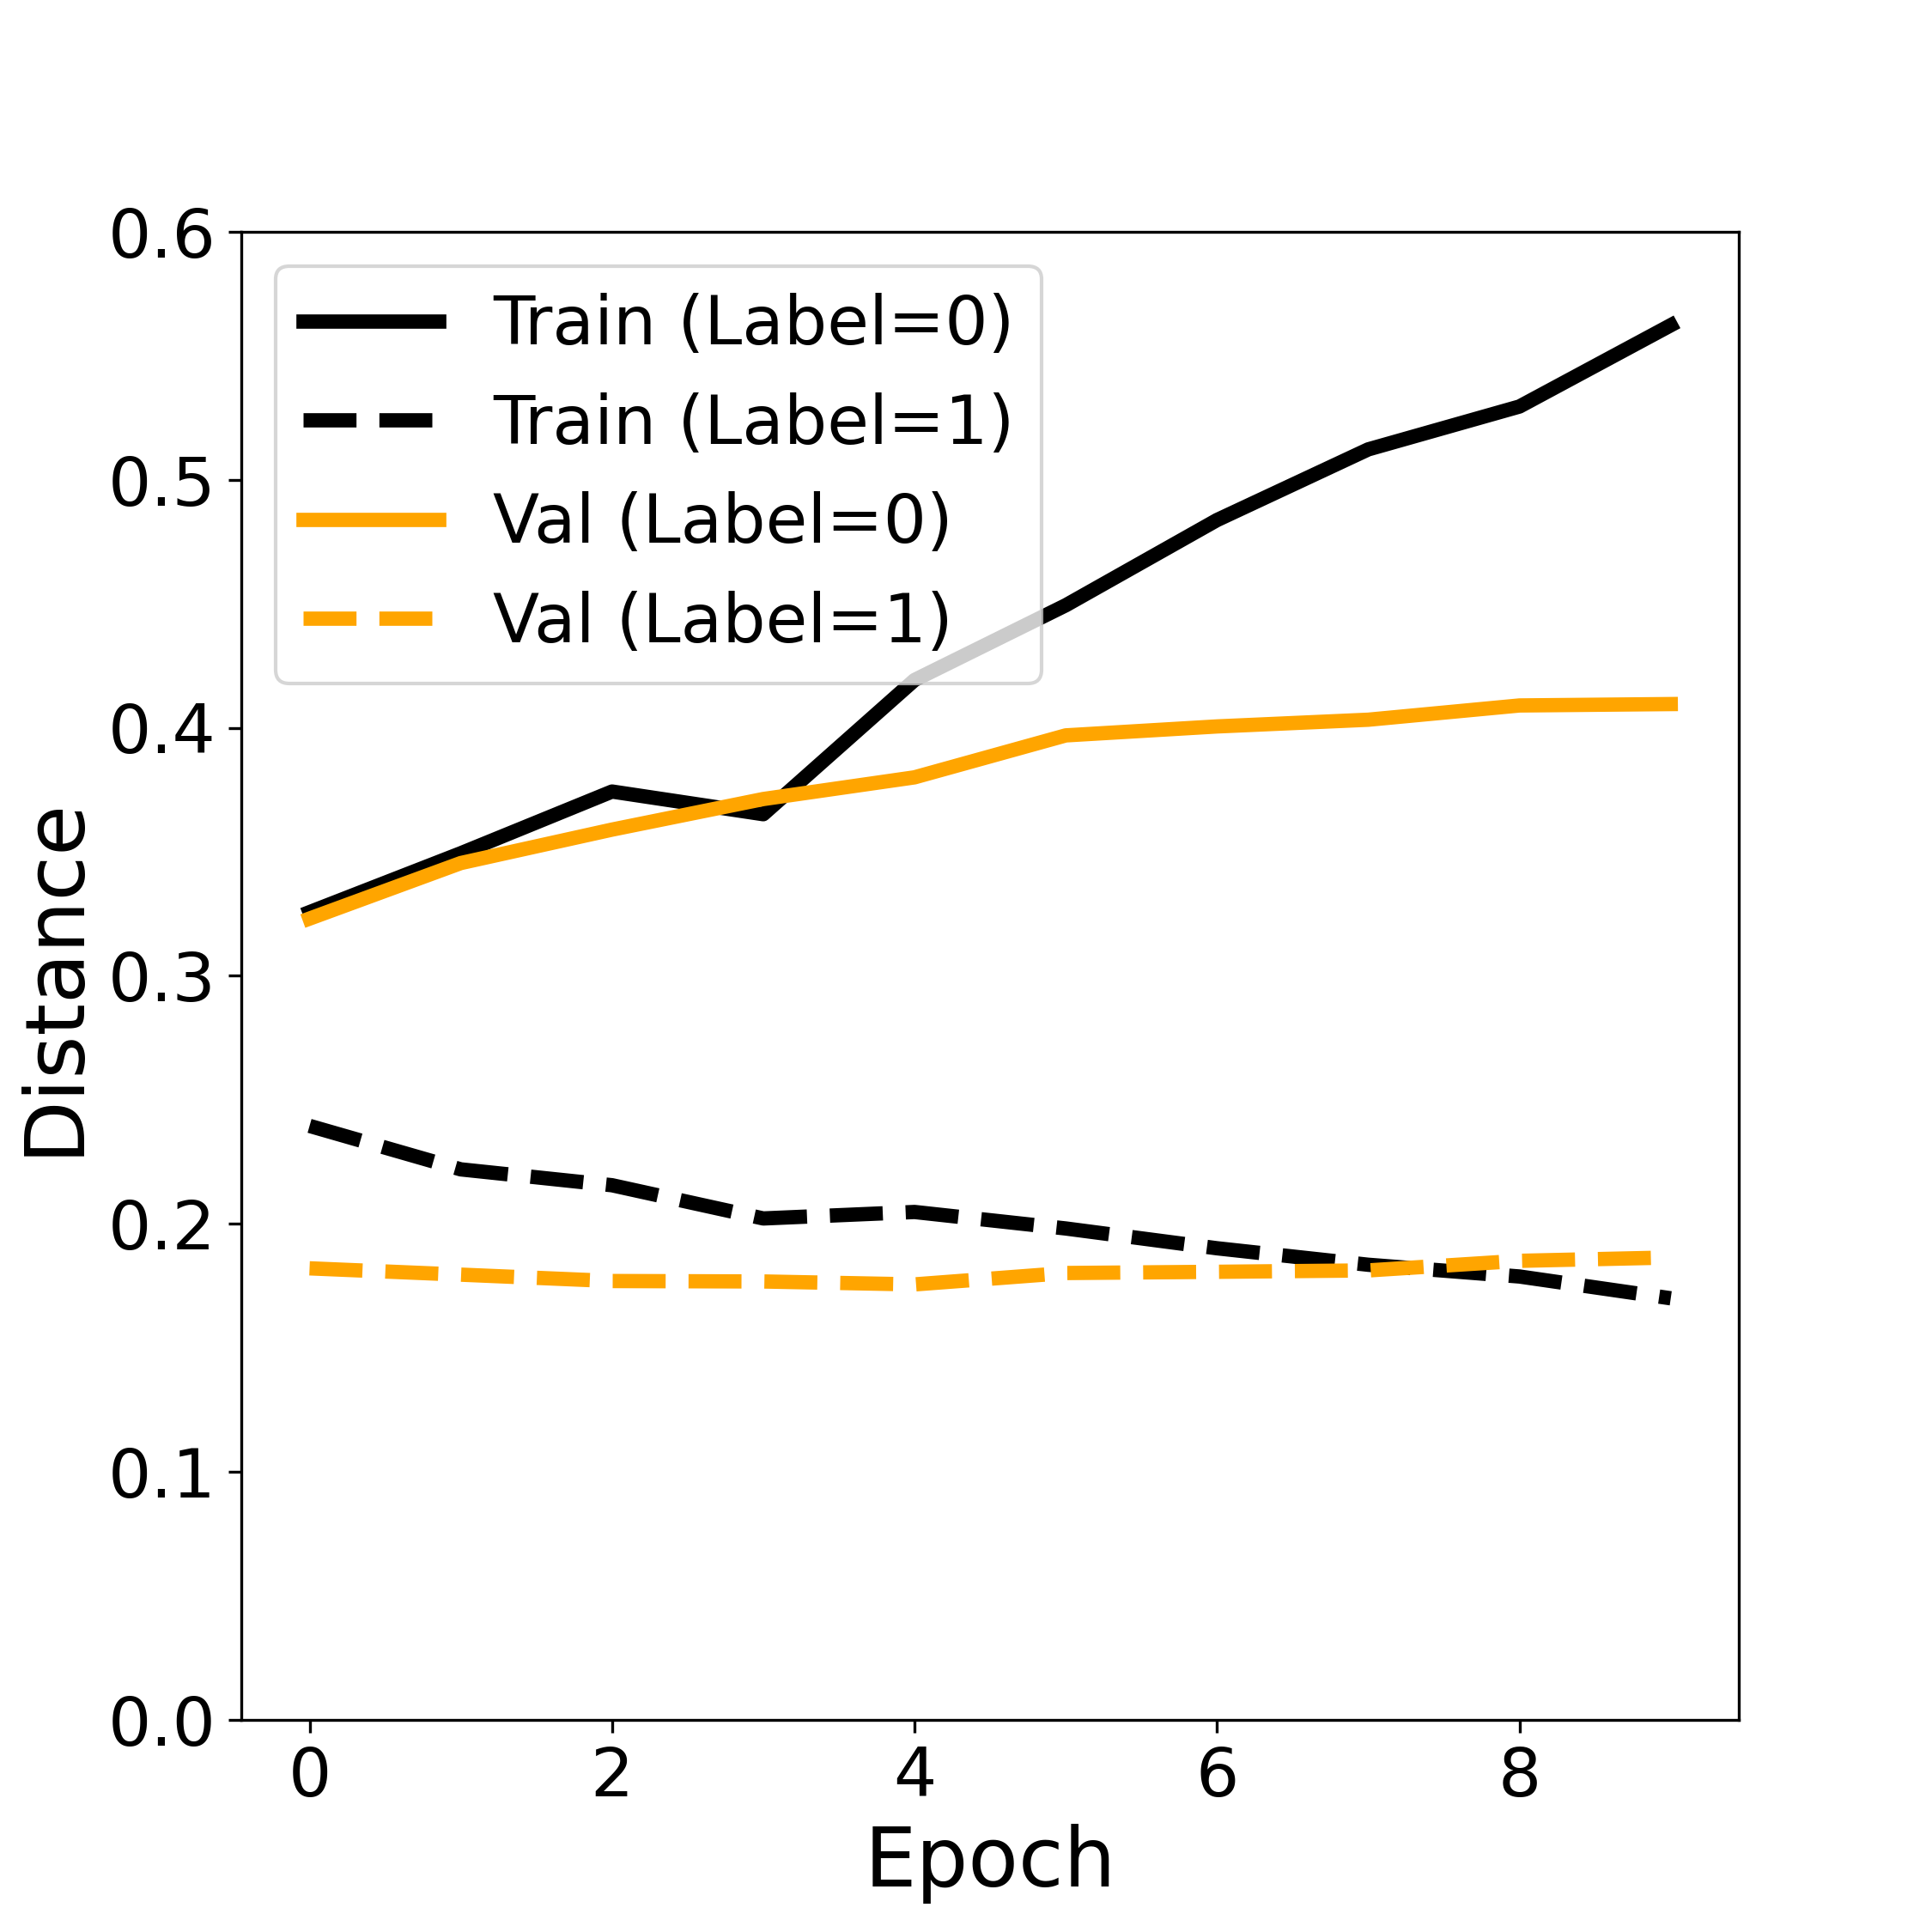
\includegraphics[width=0.33\textwidth]{Images/Distance_eps7.png}\label{fig:eps7}}
  \caption{Development of the Euclidean distance for different margin values in pairwise loss. 
  While $\epsilon=0.3$ leads to stable but low distances between positive and negative pairs, a value of $0.7$ causes noticeable differences in learning between training and validation data. 
  The values were obtained by training for ten epochs on the MRPC dataset \cite{dolan:2005}.}
  \label{fig:dist_dev}
\end{figure*}
The triplet loss is similar to the pairwise loss with the difference being that embeddings for three instead of two inputs are calculated at once.
Each of the inputs has a designated role: 
The first is the anchor $a$ against which the other two are compared. 
The second is the positive sample $x_+$ that belongs to the same distribution as the anchor, while the third is a negative sample $x_-$ from a different distribution.
Analogously, the loss is given by the sum of (1) the distance between the anchor and the positive sample, and (2) the difference between the distance to the negative sample and a pre-defined margin.
For the triplet loss, the margin was also chosen to be $\epsilon=0.5$.
\begin{equation}\begin{split}
\label{eq:tripletLoss}
    \mathcal{L}_\text{T} = \max\biggl[0, d(a, x_+)^2 - d(a, x_-)^2 + \epsilon\biggr]^2
\end{split}\end{equation}
A downside of only including one negative sample per triplet is that this input needs to be sufficiently similar to the anchor to speed up convergence.
The embeddings of negative samples that are too dissimilar will not be closer to the anchor than the margin and thus not contribute the learning process \cite{schroff:2015}.
This requires additional effort for the mining of so-called hard negatives.\\
The final loss function, InfoNCE, addresses this disadvantage by extending the loss calculation to any desired number of negative samples. 
It is an extension of Noise Contrastive Estimation \cite{gutmann:2010} and optimizes the probability of identifying the positive sample based on a score function.
Instead of using the Euclidean distance, the score $s(a, x)$ for an anchor $a$ and a candidate sample $x$ is given by the dot product of their embeddings, scaled by the temperature hyperparameter $\tau$:
\begin{equation}
\label{eq:score}
    s(a, x) =  \frac{f_\theta(a) * f_\theta(x)}{\tau}
\end{equation}
The temperature value was chosen as $\tau=0.1$ for all experiments.\\
After encoding both the anchor $a$ as well as a set $X=\{x_i\}^N_{i=1}$ of candidates with only one positive sample $x_+$, and $N-1$ negative samples, the loss is given as follows:
\begin{equation}
\label{eq:infoLoss}
    \mathcal{L}_\text{I} = -\log \biggl[
    \frac{\exp (s(a, x_+))}
    {\sum_{x \in X} \exp (s(a, x))} \biggr]
\end{equation}
This is the categorical cross-entropy loss of a classifier with the objective to match $a$ and $x_+$ \cite{he:2019}.






\section{Setup}
\label{sec:setup}
\subsection{Encoder}
\label{subsec:encoder}
As the base encoder for the experiments, we chose "all-MiniLM-L6-v2", a pre-trained sentence transformer available on Huggingface.%
\footnote{\url{www.huggingface.co/sentence-transformers/all-MiniLM-L6-v2}}
It is an adaption of the MiniLM \cite{wang:2020} with six instead of twelve layers that offers runtime advantages over other sentence transformers while still producing high quality encodings.
The model was trained on one billion sentence pairs and maps sentences or paragraphs up to a maximum of 256 words to 384-dimensional encodings that reflect the semantic content.\\
All models mentioned in the paper used this encoder as the starting point. 
Following the experiments by Khosla et al., we trained both the baseline models as well as all contrastive models using three different optimizers: SGD with momentum, RMSPRop, and LARS \cite{khosla:2020}.
This leads to three baseline models, one for each optimizer, and nine contrastive models, because each contrastive loss was paired with each optimizer.


\subsection{Training data}
In order to cater to the specifics of the different loss functions, a custom dataset was created from the publicly available PAWS \cite{zhang2019paws} and Parabank \cite{hu2019parabank}. \\
PAWS contains two subsets, sourced from Wikipedia and duplicate questions from Quora, and contains paraphrases as well as pairs of similar sentences which are not actually paraphrases.\\
Parabank consists of paraphrases automatically generated through lexically constrained machine translation and does not contain similar sentences that are not paraphrases.\\
The final structure of the contrastive dataset is as follows: "sentence1" contains the anchor sentence, "sentence2" contains the paraphrase, and columns "sentence\{3-6\}" contain sentences which are similar in n-grams to the anchor, but are not paraphrases.
To achieve this, we generated an index using PyTerrier \footnote{https://pyterrier.readthedocs.io/en/latest/}, an information retrieval library API for Python.
Indices were generated for each dataset and each split (train, validation, test) separately, to avoid leaking sentences between the sets.
We then used each anchor from the paraphrase pairs to retrieve the most similar sentences in the same subset.
Those sentences are similar in terms of n-gram overlap but not necessarily in semantics.\\
To exclude sentences from the negative samples which are too similar or actual paraphrases to the anchor, we did not use sentences for which the retrieval score was over a certain threshold.
This threshold was chosen individually for each anchor, based on the retrieval score $r_p$ the exact same sentence got from the retrieval model.
The next best sentence is added as a negative sample, if it's retrieval score is below $0.7 \times r_p$. 
If not, the new value for $r_p$ is set to the current retrieval score, and the next sentence is evaluated.
This excludes the same sentence from being chosen as a negative, as well as the paraphrase and possible other sentences which might have exactly the same semantic meaning, which could not be verified for each result.
The threshold of $0.7$ was chosen heuristically, based on evaluating a small set of retrieval results. \\\\
Sentence pairs in the original datasets that are flagged as non-paraphrases were not used in the contrastive dataset, since it would have been necessary to created new paraphrases for those sentences.
We experimented with different paraphrasing models from Huggingface, but noticed to many generated paraphrases which were not actual paraphrases, so we decided not to include them in the final dataset.
An additional hurdle was the long processing time needed to generate paraphrases.\\\\

The total dataset size and the origin of the used sentences are shown in Table \ref{tab:dataset}.
Of each dataset and corresponding split a maximum of 50000 sentence pairs are used.
Of those 50000, all non-paraphrase pairs are discarded. 
For the remaining pairs, negative samples are retrieved.
If not enough negatives can be retrieved, the sentence pair is discarded.
The splits for all PAWS related datasets are taken from the official splits, while for parabank the first 50000 sentences were used for train and the next 5000 for validation.\\
This results is a dataset containing 92303 data points in total, split in about 83-13-4 (train-validation-test).

% Please add the following required packages to your document preamble:
% \usepackage{graphicx}
\begin{table*}[!]
\resizebox{\textwidth}{!}{
\begin{tabular}{c|ccccc|c}
 & paws\_labeled\_final & paws\_unlabeled\_final & paws\_labeled\_swap & paws\_quora & parabank\_small\_diverse & total \\ \hline
train      & 21203 & 23851 & 2795 & 3170 & 25843 & 76862 \\
validation & 3492  & 4944  &      &      & 3329  & 11765 \\
test       & 3497  &       &      & 179  &       & 3676  \\ \hline
total      & 28192 & 28795 & 2795 & 3349 & 29172 & 92303
\end{tabular}%
}
\caption{Origin datasets of used anchors and paraphrases for contrastive dataset. Also shows, train, validation, test split.}
\label{tab:dataset}
\end{table*}



\subsection{Evaluation data}
The models' performance on the task of text alignment was evaluated on the PAN-13 dataset \cite{potthast:2013e}.
%Todo: Cecilia

\section{Experiment}
\label{sec:experiment}
As a first step in the training process, Bayesian hyperparameter sweeps were conducted using the services offered by the Weights and Biases platform.%
\footnote{\url{www.wandb.ai}}
In order to avoid train-test leakage, the sweeps were done on MRPC, a small dataset that contains entirely different sentence pairs from those in the training corpus \cite{dolan:2005}.
The identified hyperparameter values are summarized in Table \ref{tab:hyperparam}.\\
\begin{table*}[!tbp]
\centering
\begin{tabular}{llllll}
\hline
\textbf{Configuration} & \textbf{Learning Rate} & \textbf{Momentum} & \textbf{Alpha} & \textbf{Epsilon} & \textbf{Trust}\\
\hline
Base\_SGD           & 0.0050 & 0.70 &    - &      - & -\\
Base\_RMSProp       & 0.0020 & 0.80 & 0.85 & 1.5e-9 & -\\
Base\_LARS          & 0.2850 & 0.30 &    - & 1.0e-8 & 0.00125\\
Pairwise\_SGD       & 0.0055 & 0.70 &    - &      - & -\\
Pairwise\_RMSProp   & 0.0001 & 0.10 & 0.95 & 1.0e-9 & -\\
Pairwise\_LARS      & 0.0075 & 0.15 &    - & 6.0e-9 & 0.00500\\
Triplet\_SGD        & 0.0015 & 0.75 &    - &      - & -\\
Triplet\_RMSProp    & 0.0015 & 0.90 & 0.90 & 1.0e-8 & -\\
Triplet\_LARS       & 0.0300 & 0.85 &    - & 1.0e-8 & 0.00100\\
InfoNCE\_SGD        & 0.0030 & 0.55 &    - &      - & -\\
InfoNCE\_RMSProp    & 0.0040 & 0.50 & 0.85 & 3.5e-8 & -\\
InfoNCE\_LARS       & 0.0850 & 0.00 &    - & 1.5e-9 & 0.00050\\
\hline
\end{tabular}
\caption{\label{tab:hyperparam}
Hyperparameter values for each configuration.
The values were obtained through Bayesian sweeps on the GLUE MRPC dataset \cite{dolan:2005, wang:2018}. After running 50 sweeps for each configuration, the five sweeps with the lowest validation loss were used to select the parameter values.  
}
\end{table*}
The second step consisted of training each of the nine contrastive optimizer-loss-configurations mentioned in \ref{subsec:encoder} on our custom training set.
A visualization of the loss developments for each function can be found in Figures \ref{fig:pairOpt}, \ref{fig:tripletOpt}, and \ref{fig:infoOpt} in the appendix.
SGD achieved the best performance for the pairwise loss, whereas LARS outperformed the other optimizers for triplet loss and InfoNCE. %Todo: Update based on results
The three encoders trained with these optimizers were then selected to train a classifier on top.\\
The third and final training step involved training the classifiers, three baseline models as well as three pre-trained contrastive models.
%Todo: Describe the results and visualize the loss curves in graphs for each loss function.

\subsection{Evaluation}
%Todo: Cecilia
%- Preparation for the evaluation (Dataset, Pladget Score)
%- Results of the evaluation



\section{Discussion}
\label{sec:discussion}
%Todo: Desribe the results

\section{Conclusion}
\label{sec:conclusion}





% Entries for the entire Anthology, followed by custom entries
\bibliography{anthology,custom}
\bibliographystyle{acl_natbib}

\appendix
\section{Appendix}
\label{sec:appendix}

\begin{figure*}[!tbp]
  \centering
  \subfloat[Loss on the train set]{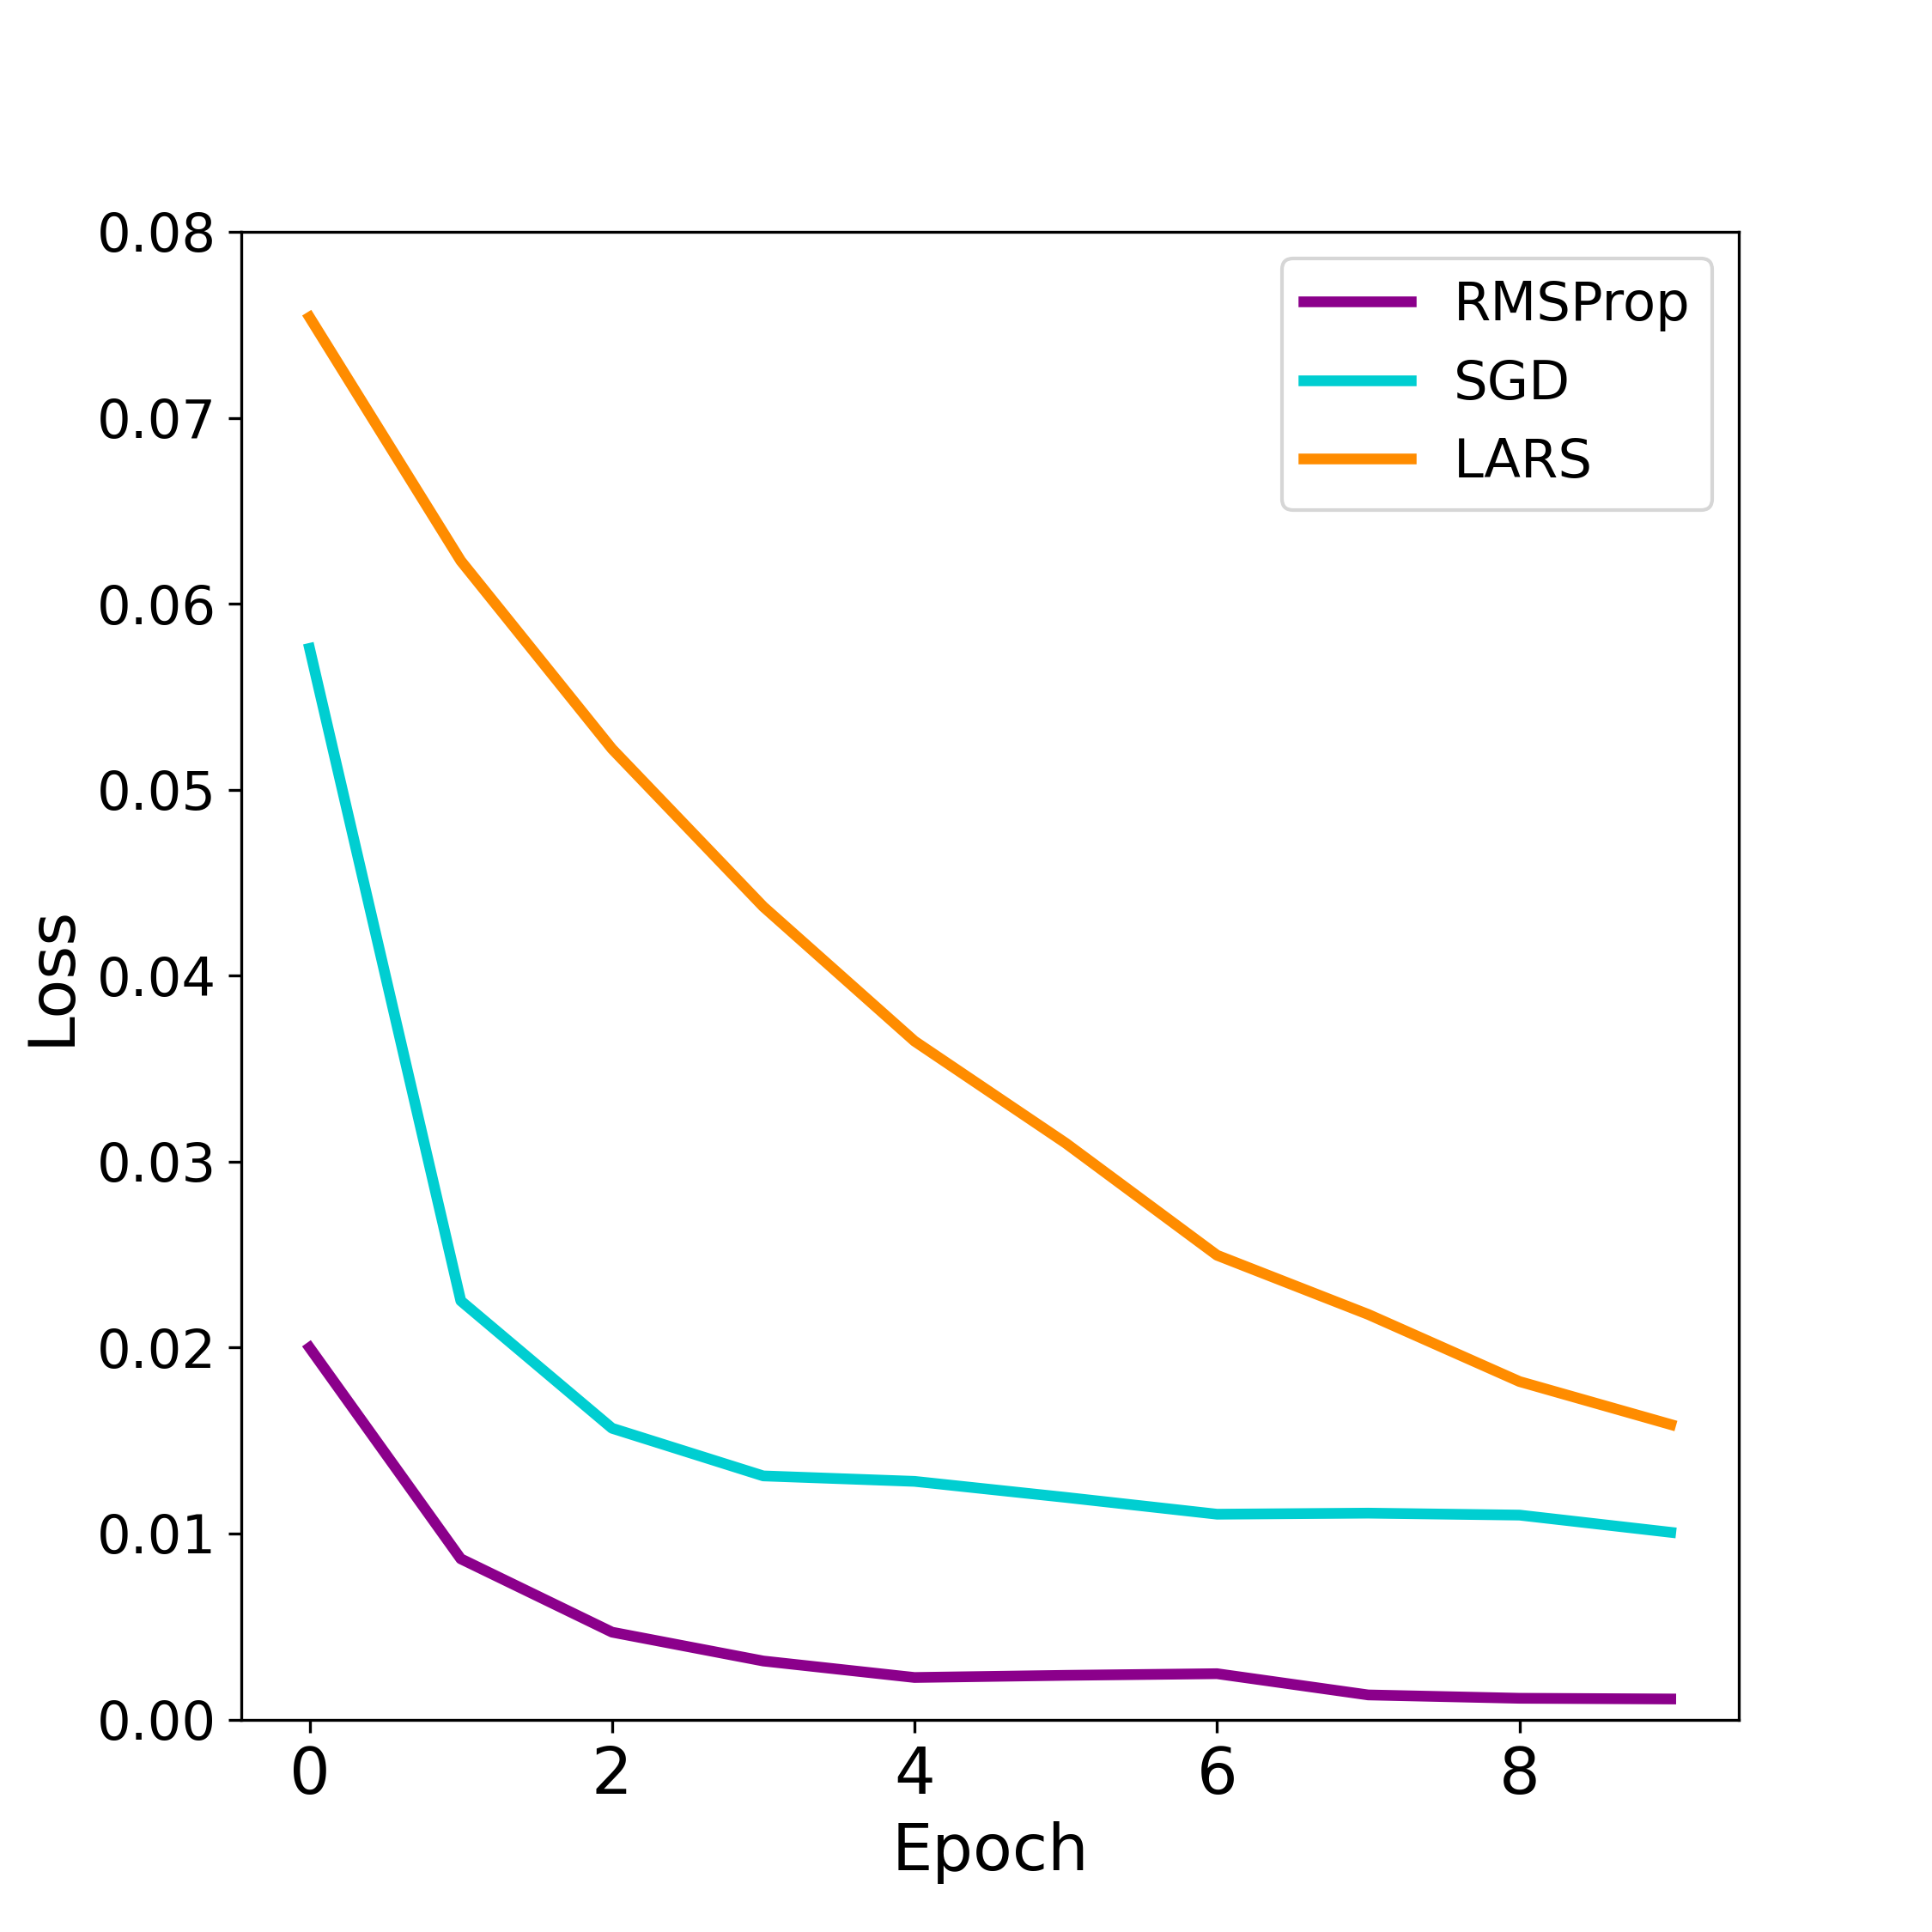
\includegraphics[width=0.45\textwidth]{Images/Pairwise_Train.png}\label{fig:pairOptTrain}}
  \subfloat[Loss on the validation set]{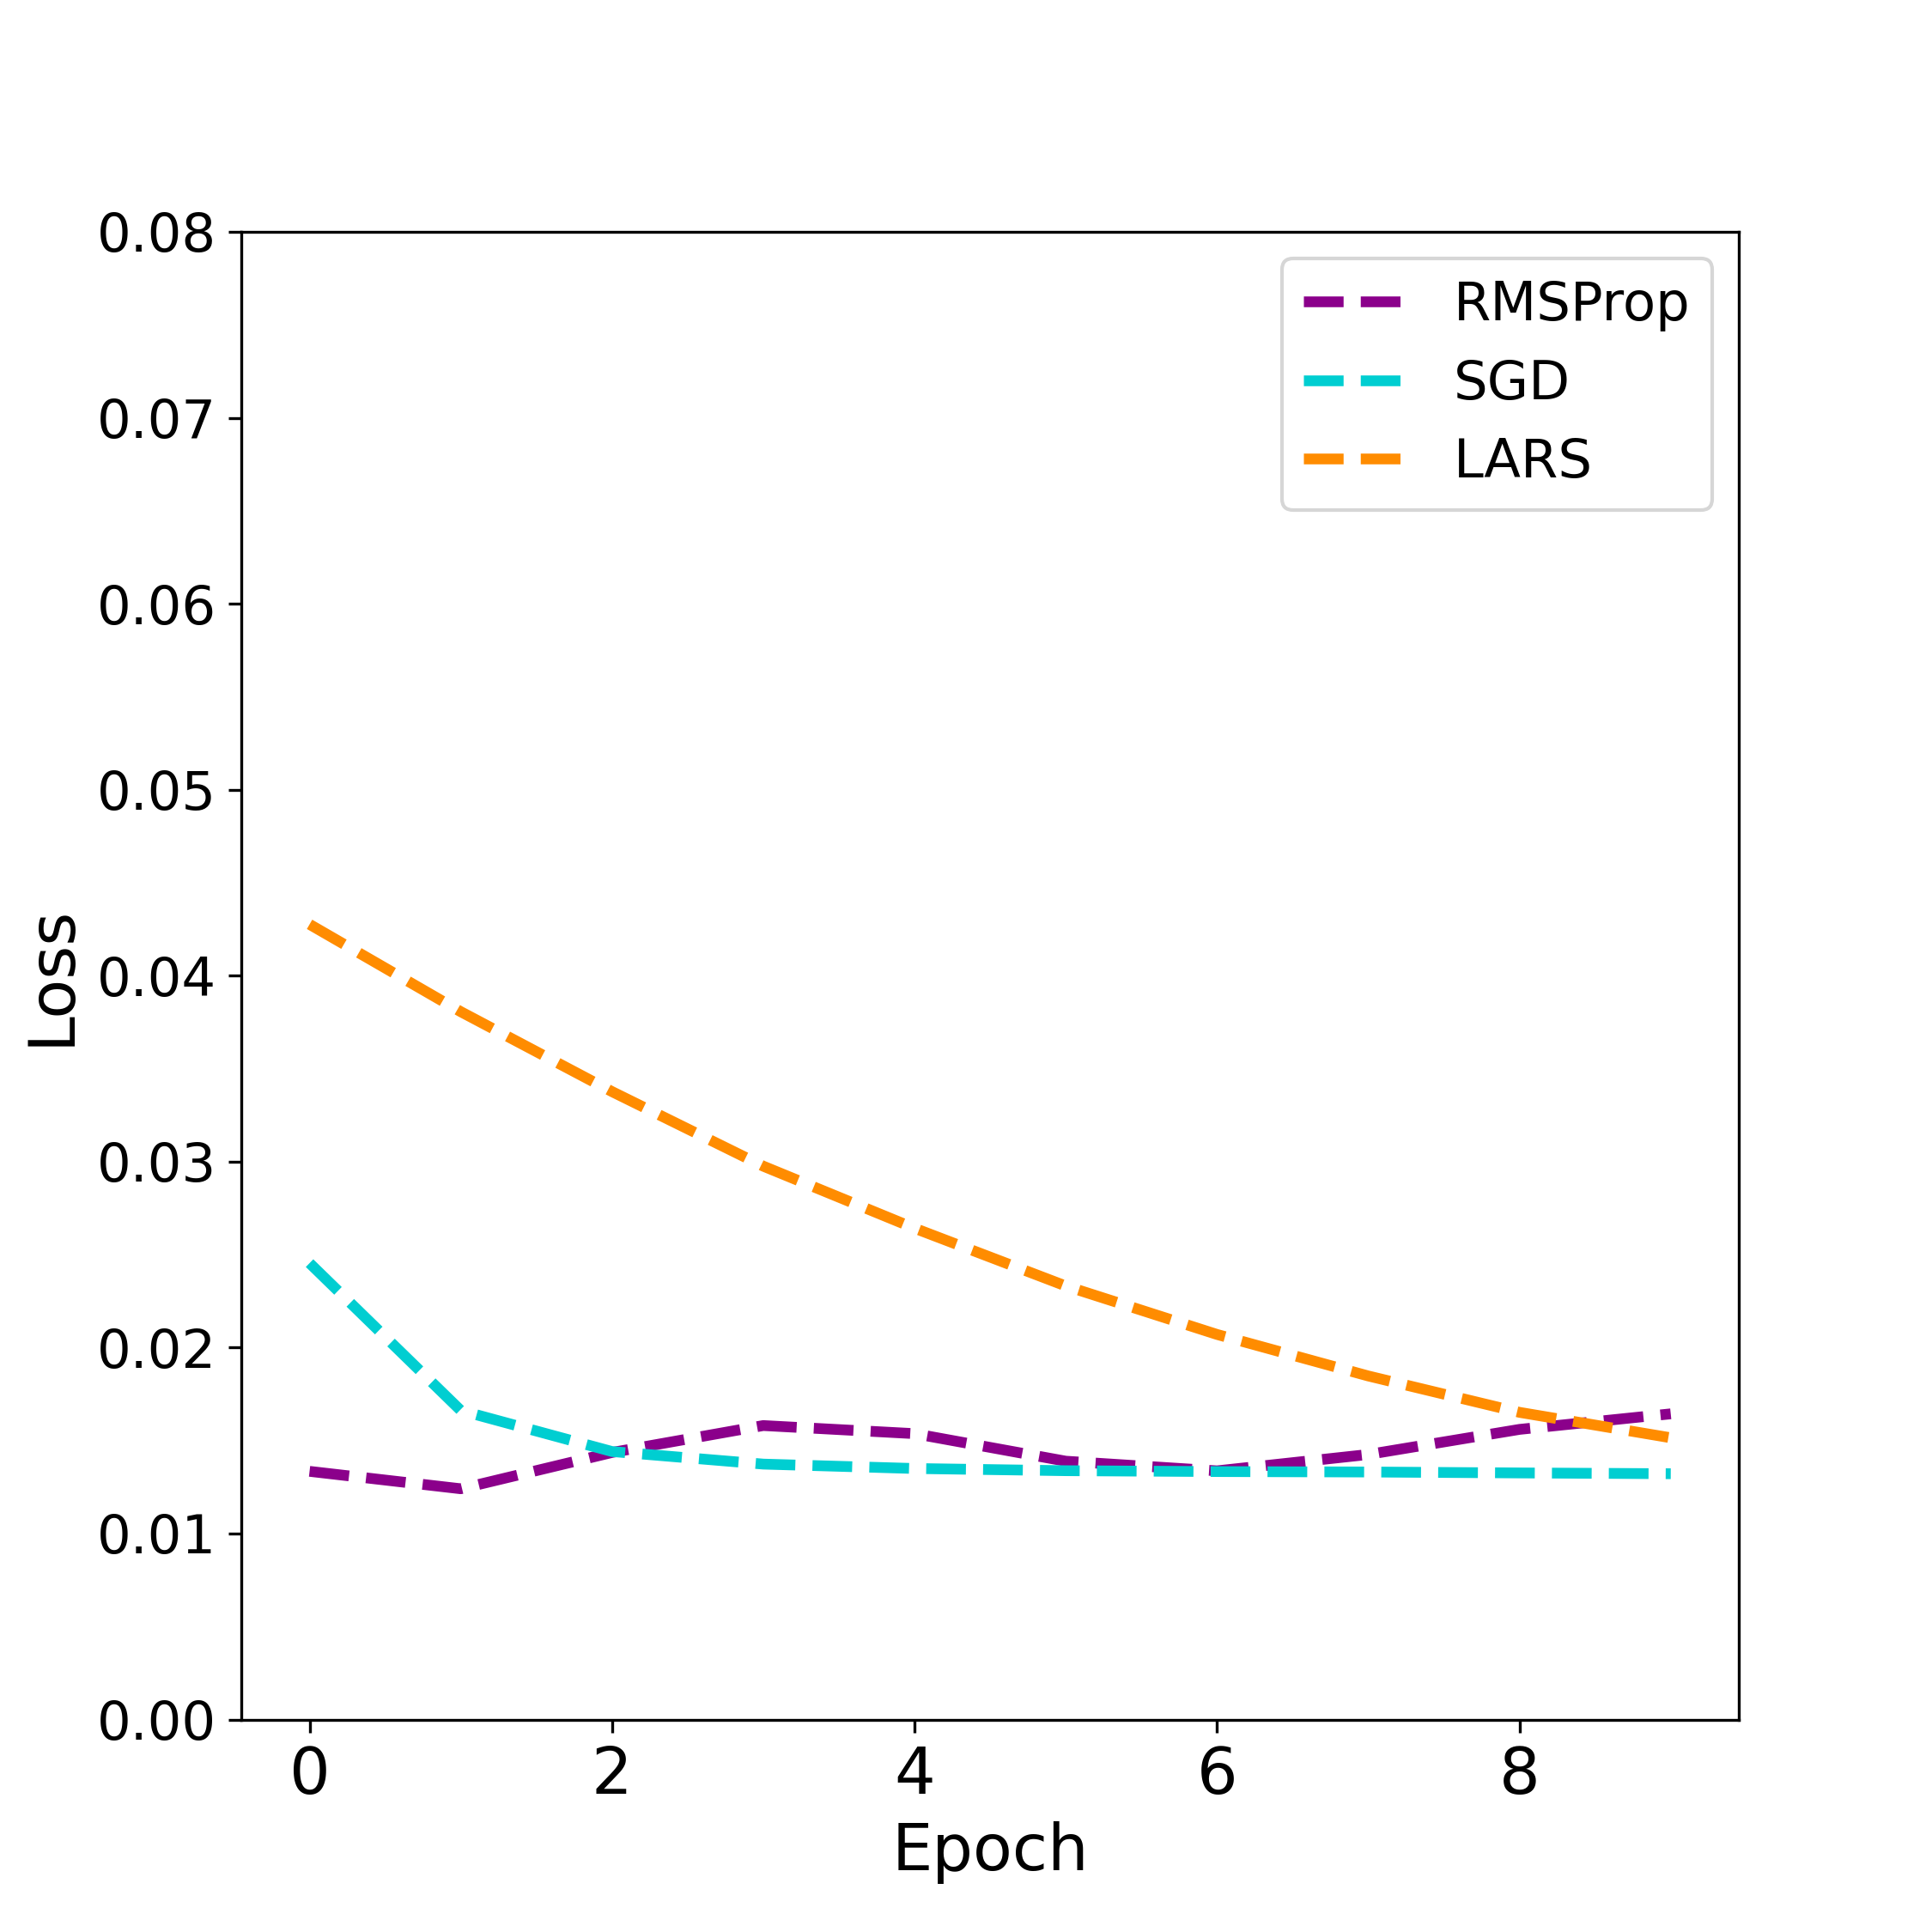
\includegraphics[width=0.45\textwidth]{Images/Pairwise_Validation.png}
  \label{fig:pairOptVal}}
  \caption{Pairwise loss for different optimizers.}
  \label{fig:pairOpt}
\end{figure*}

\begin{figure*}[!tbp]
  \centering
  \subfloat[Loss on the train set]{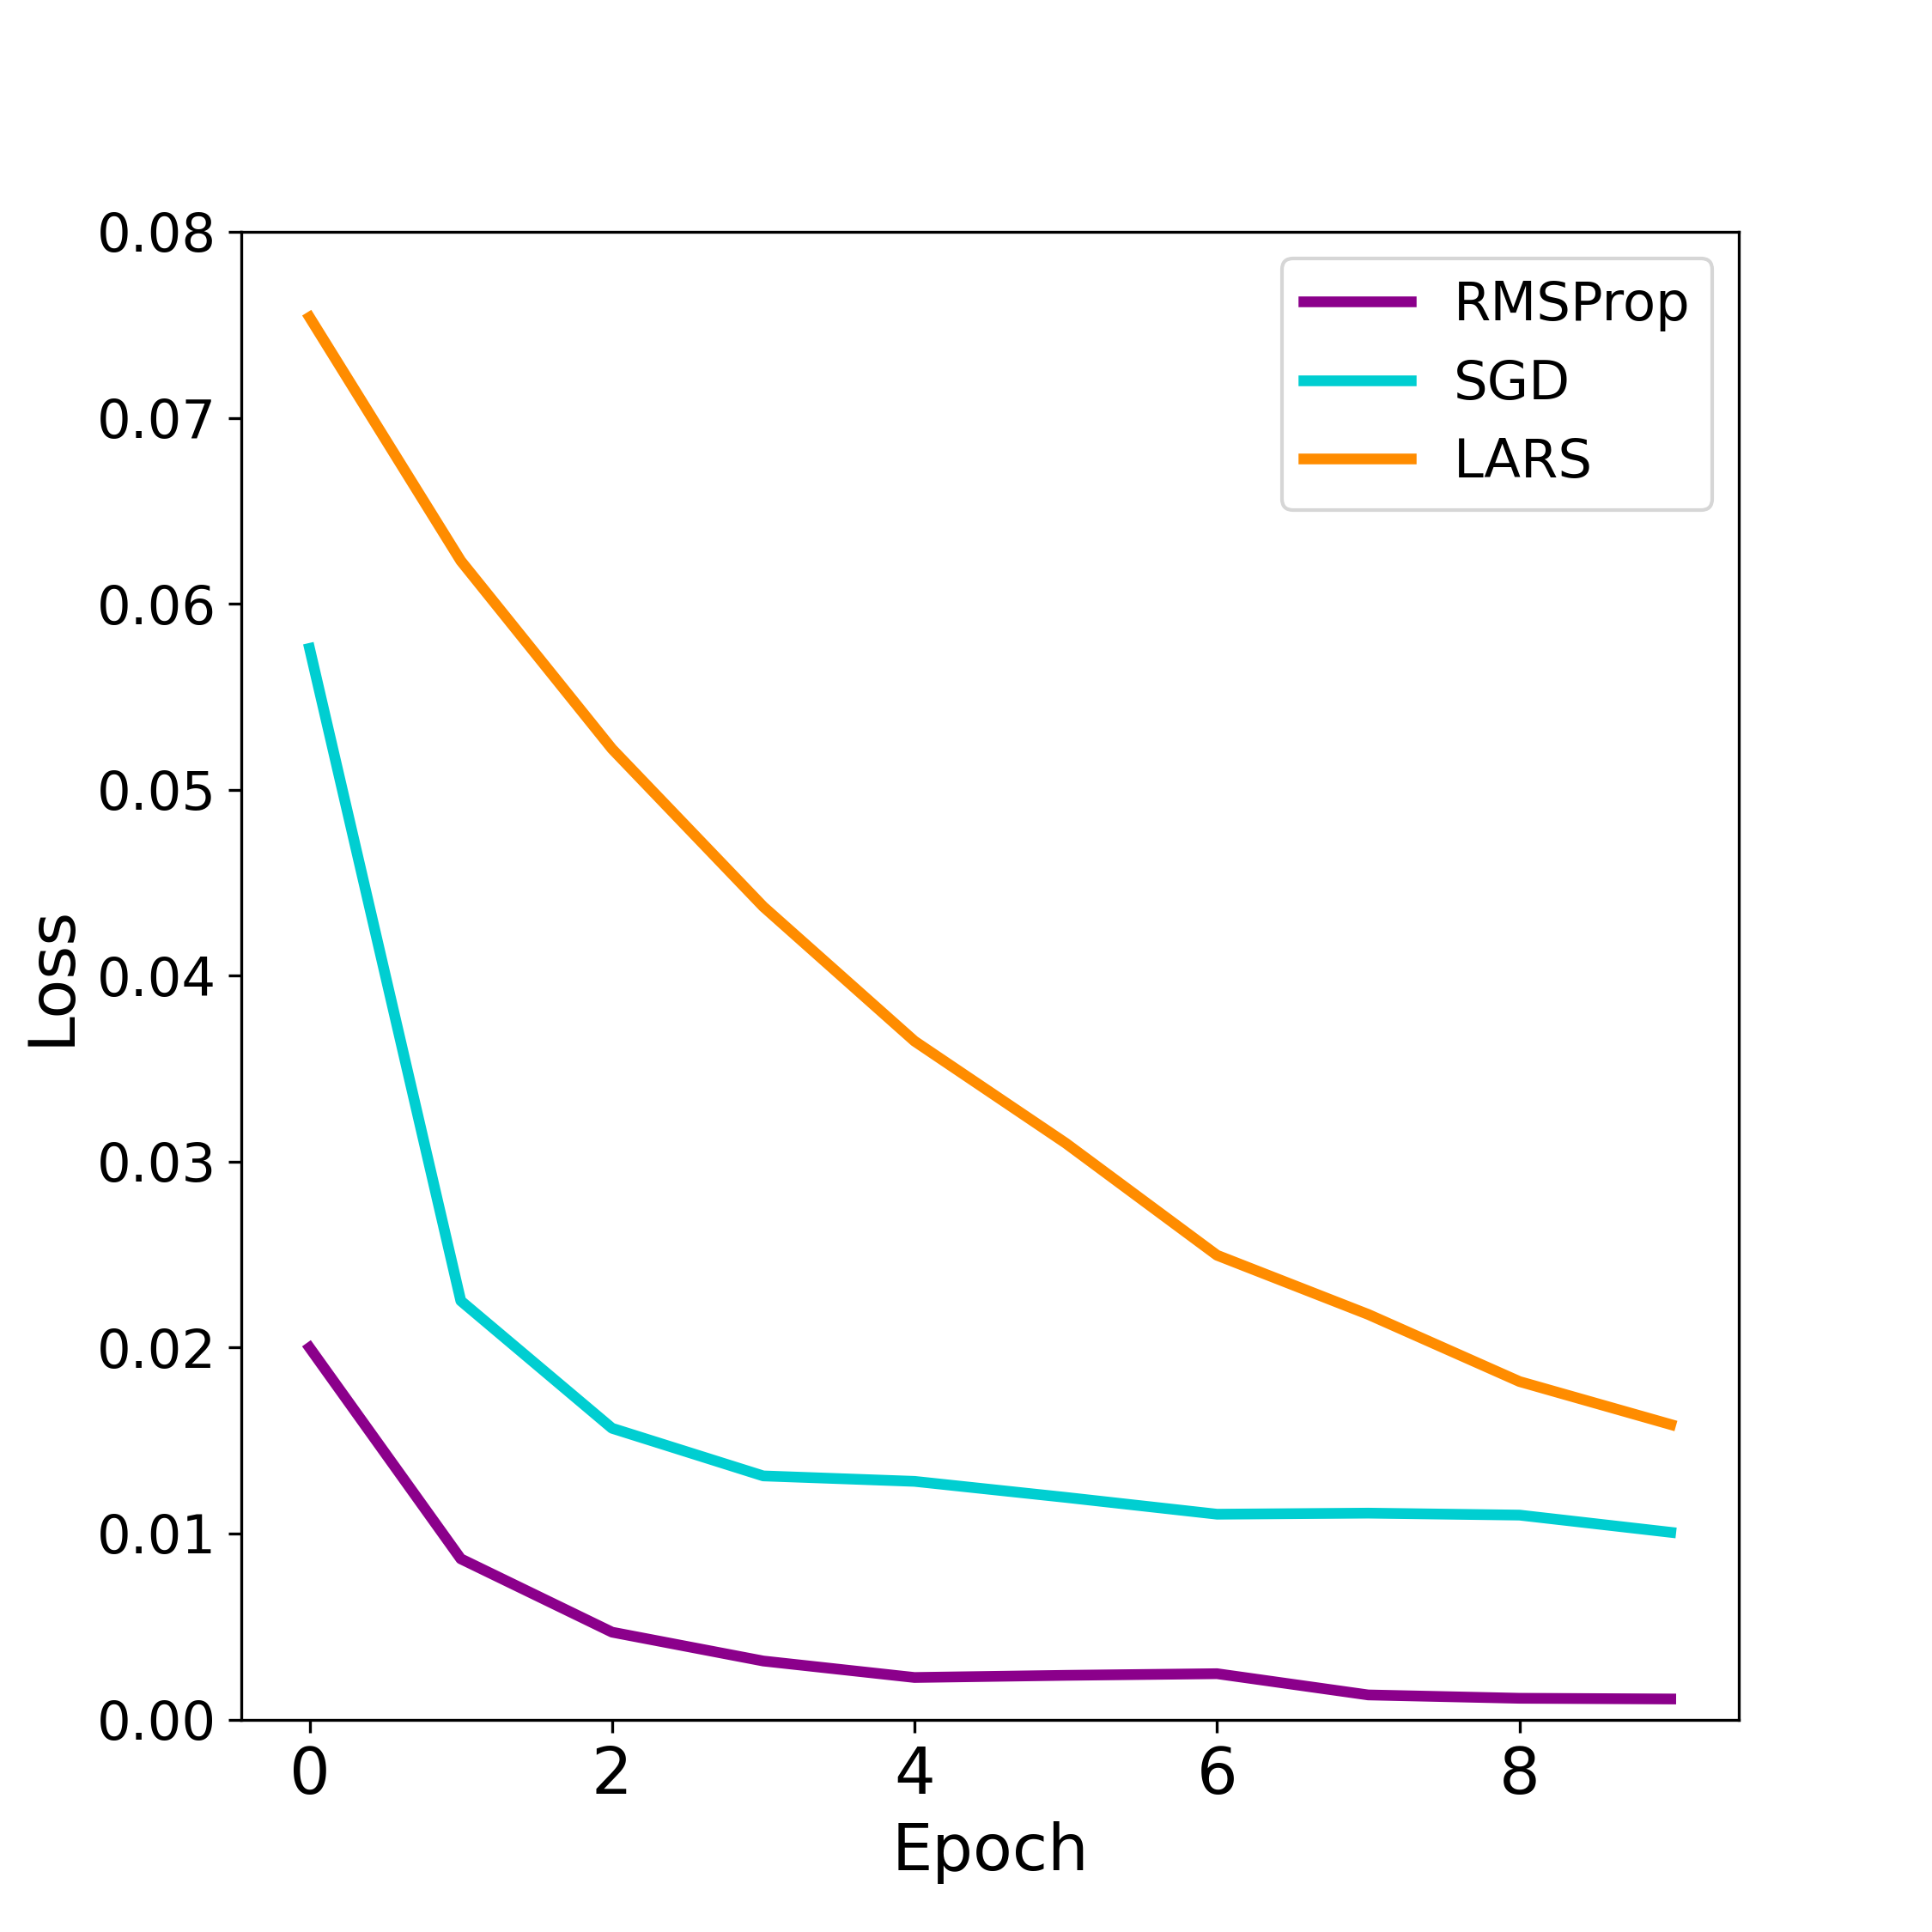
\includegraphics[width=0.45\textwidth]{Images/Pairwise_Train.png}\label{fig:tripletOptTrain}}
  \subfloat[Loss on the validation set]{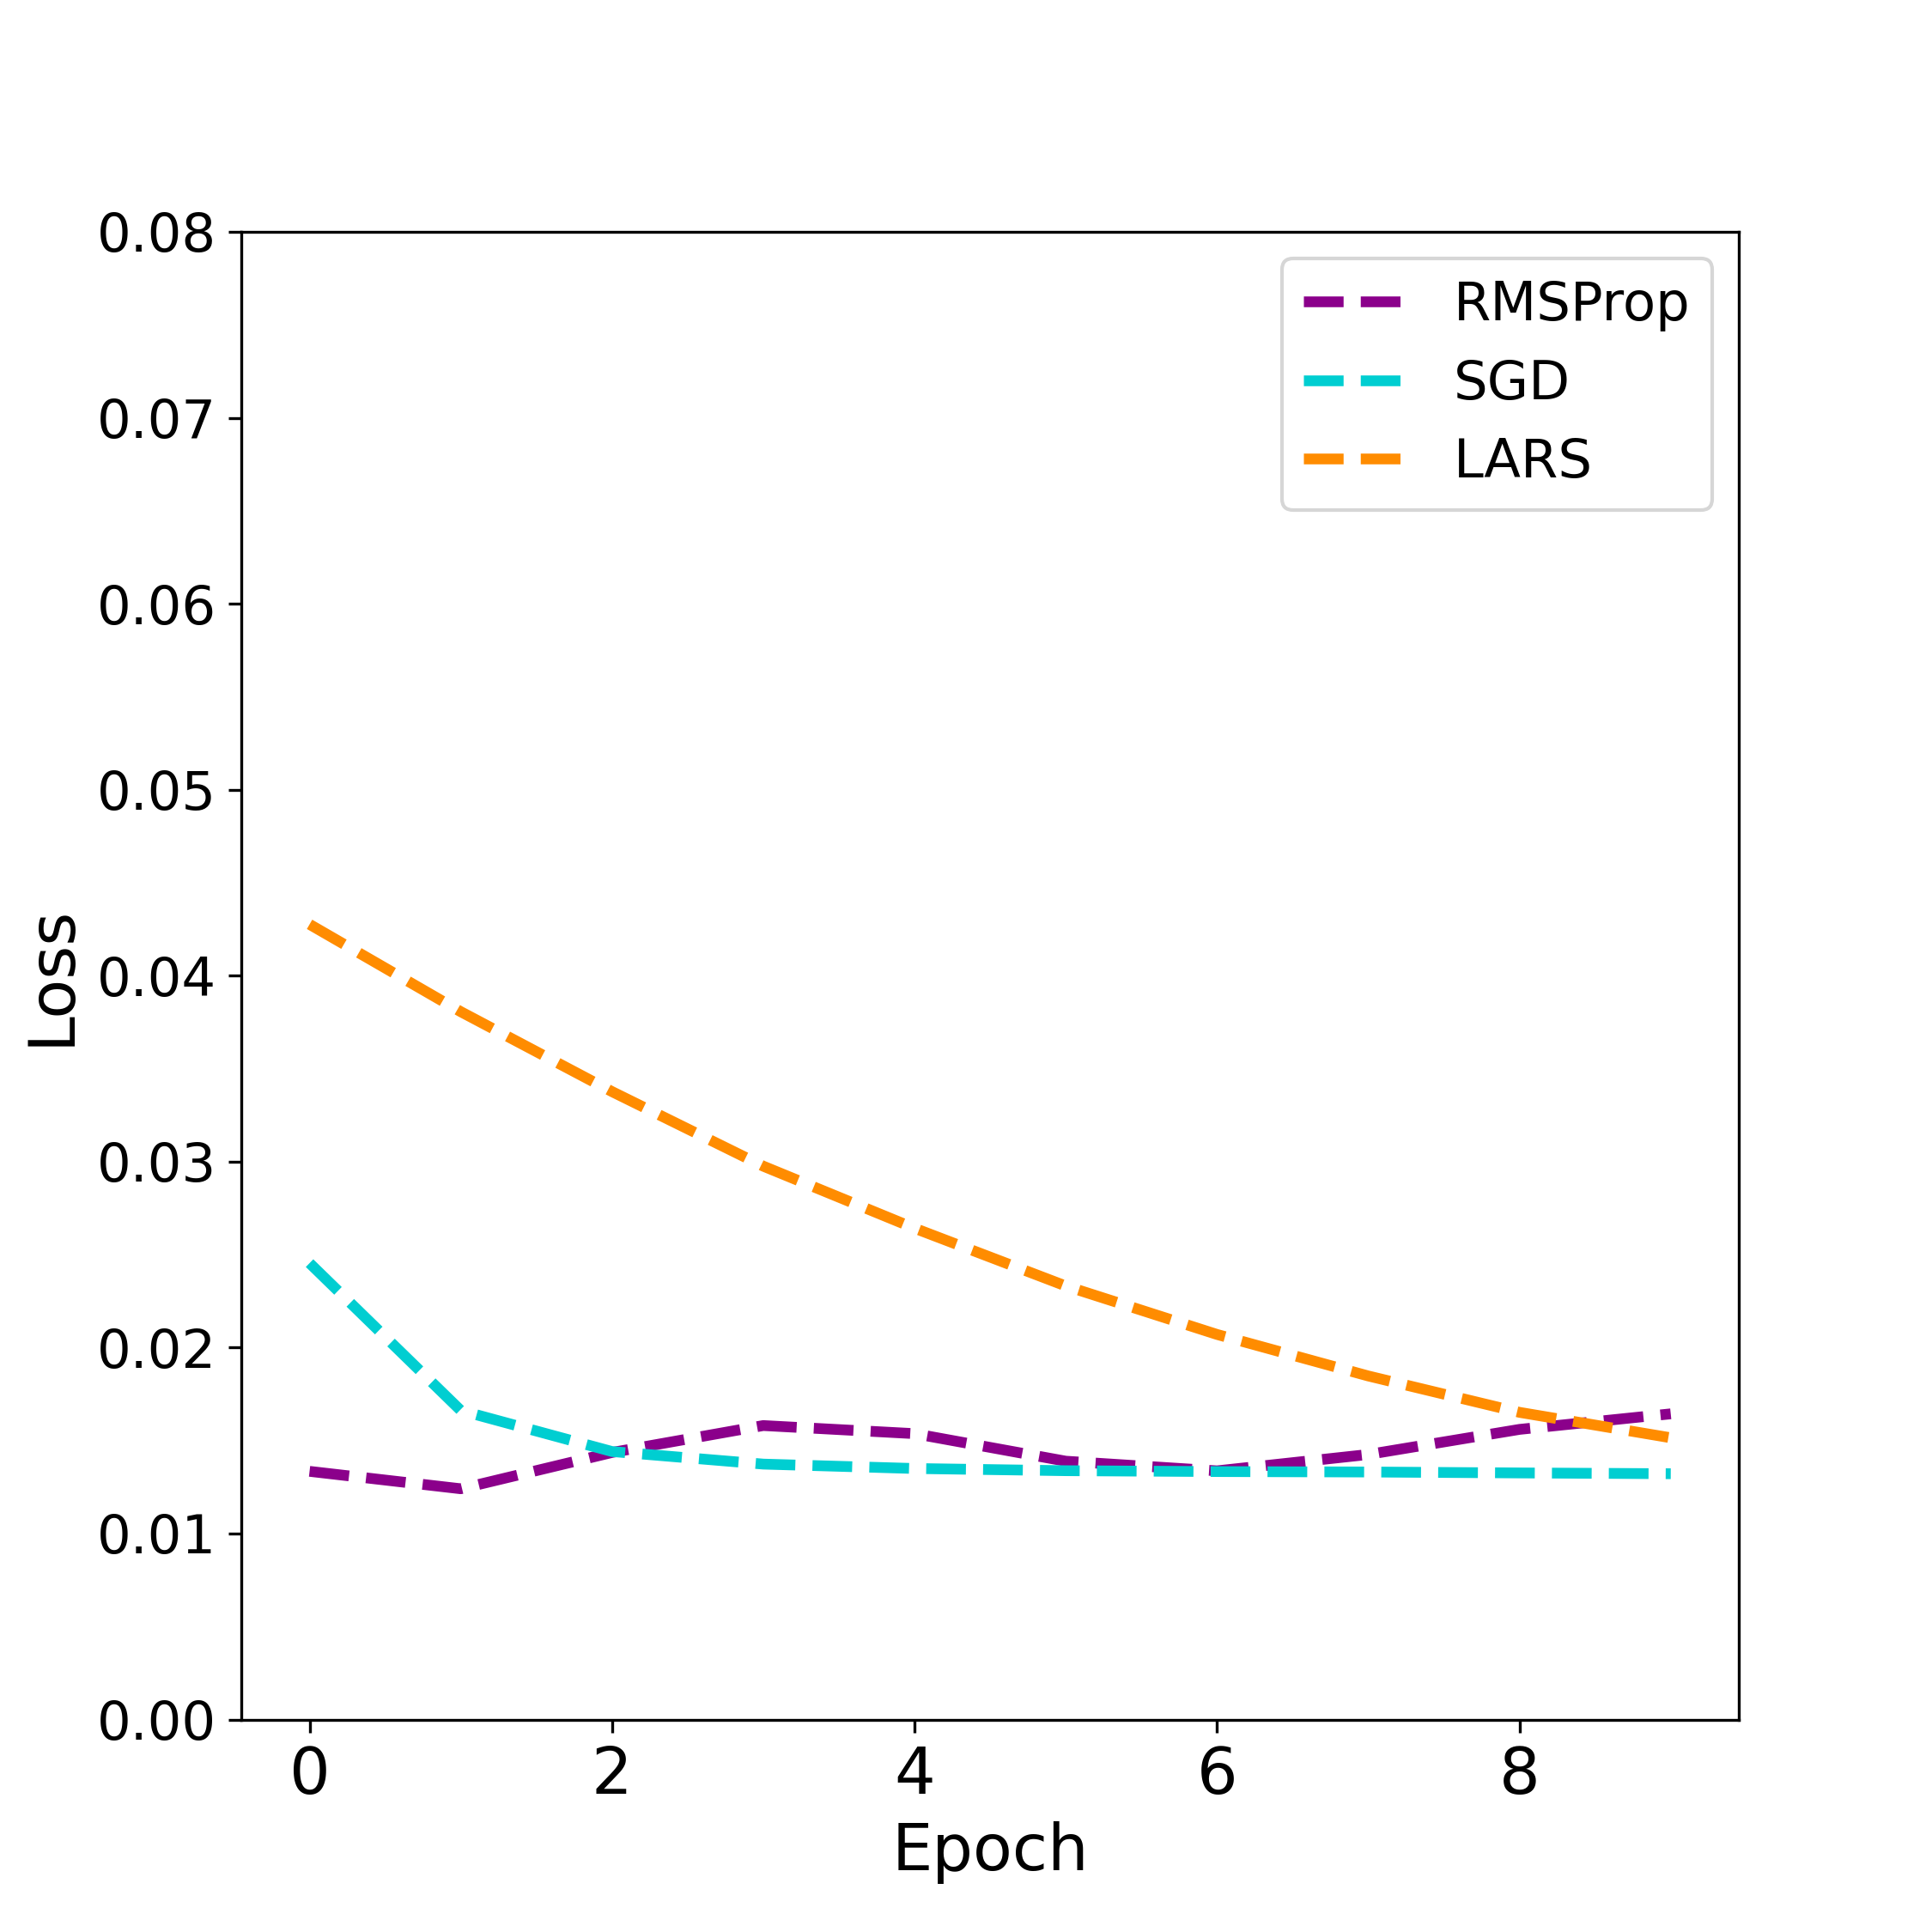
\includegraphics[width=0.45\textwidth]{Images/Pairwise_Validation.png}
  \label{fig:tripletOptVal}}
  \caption{Triplet loss for different optimizers.}
  \label{fig:tripletOpt}
\end{figure*}

\begin{figure*}[!tbp]
  \centering
  \subfloat[Loss on the train set]{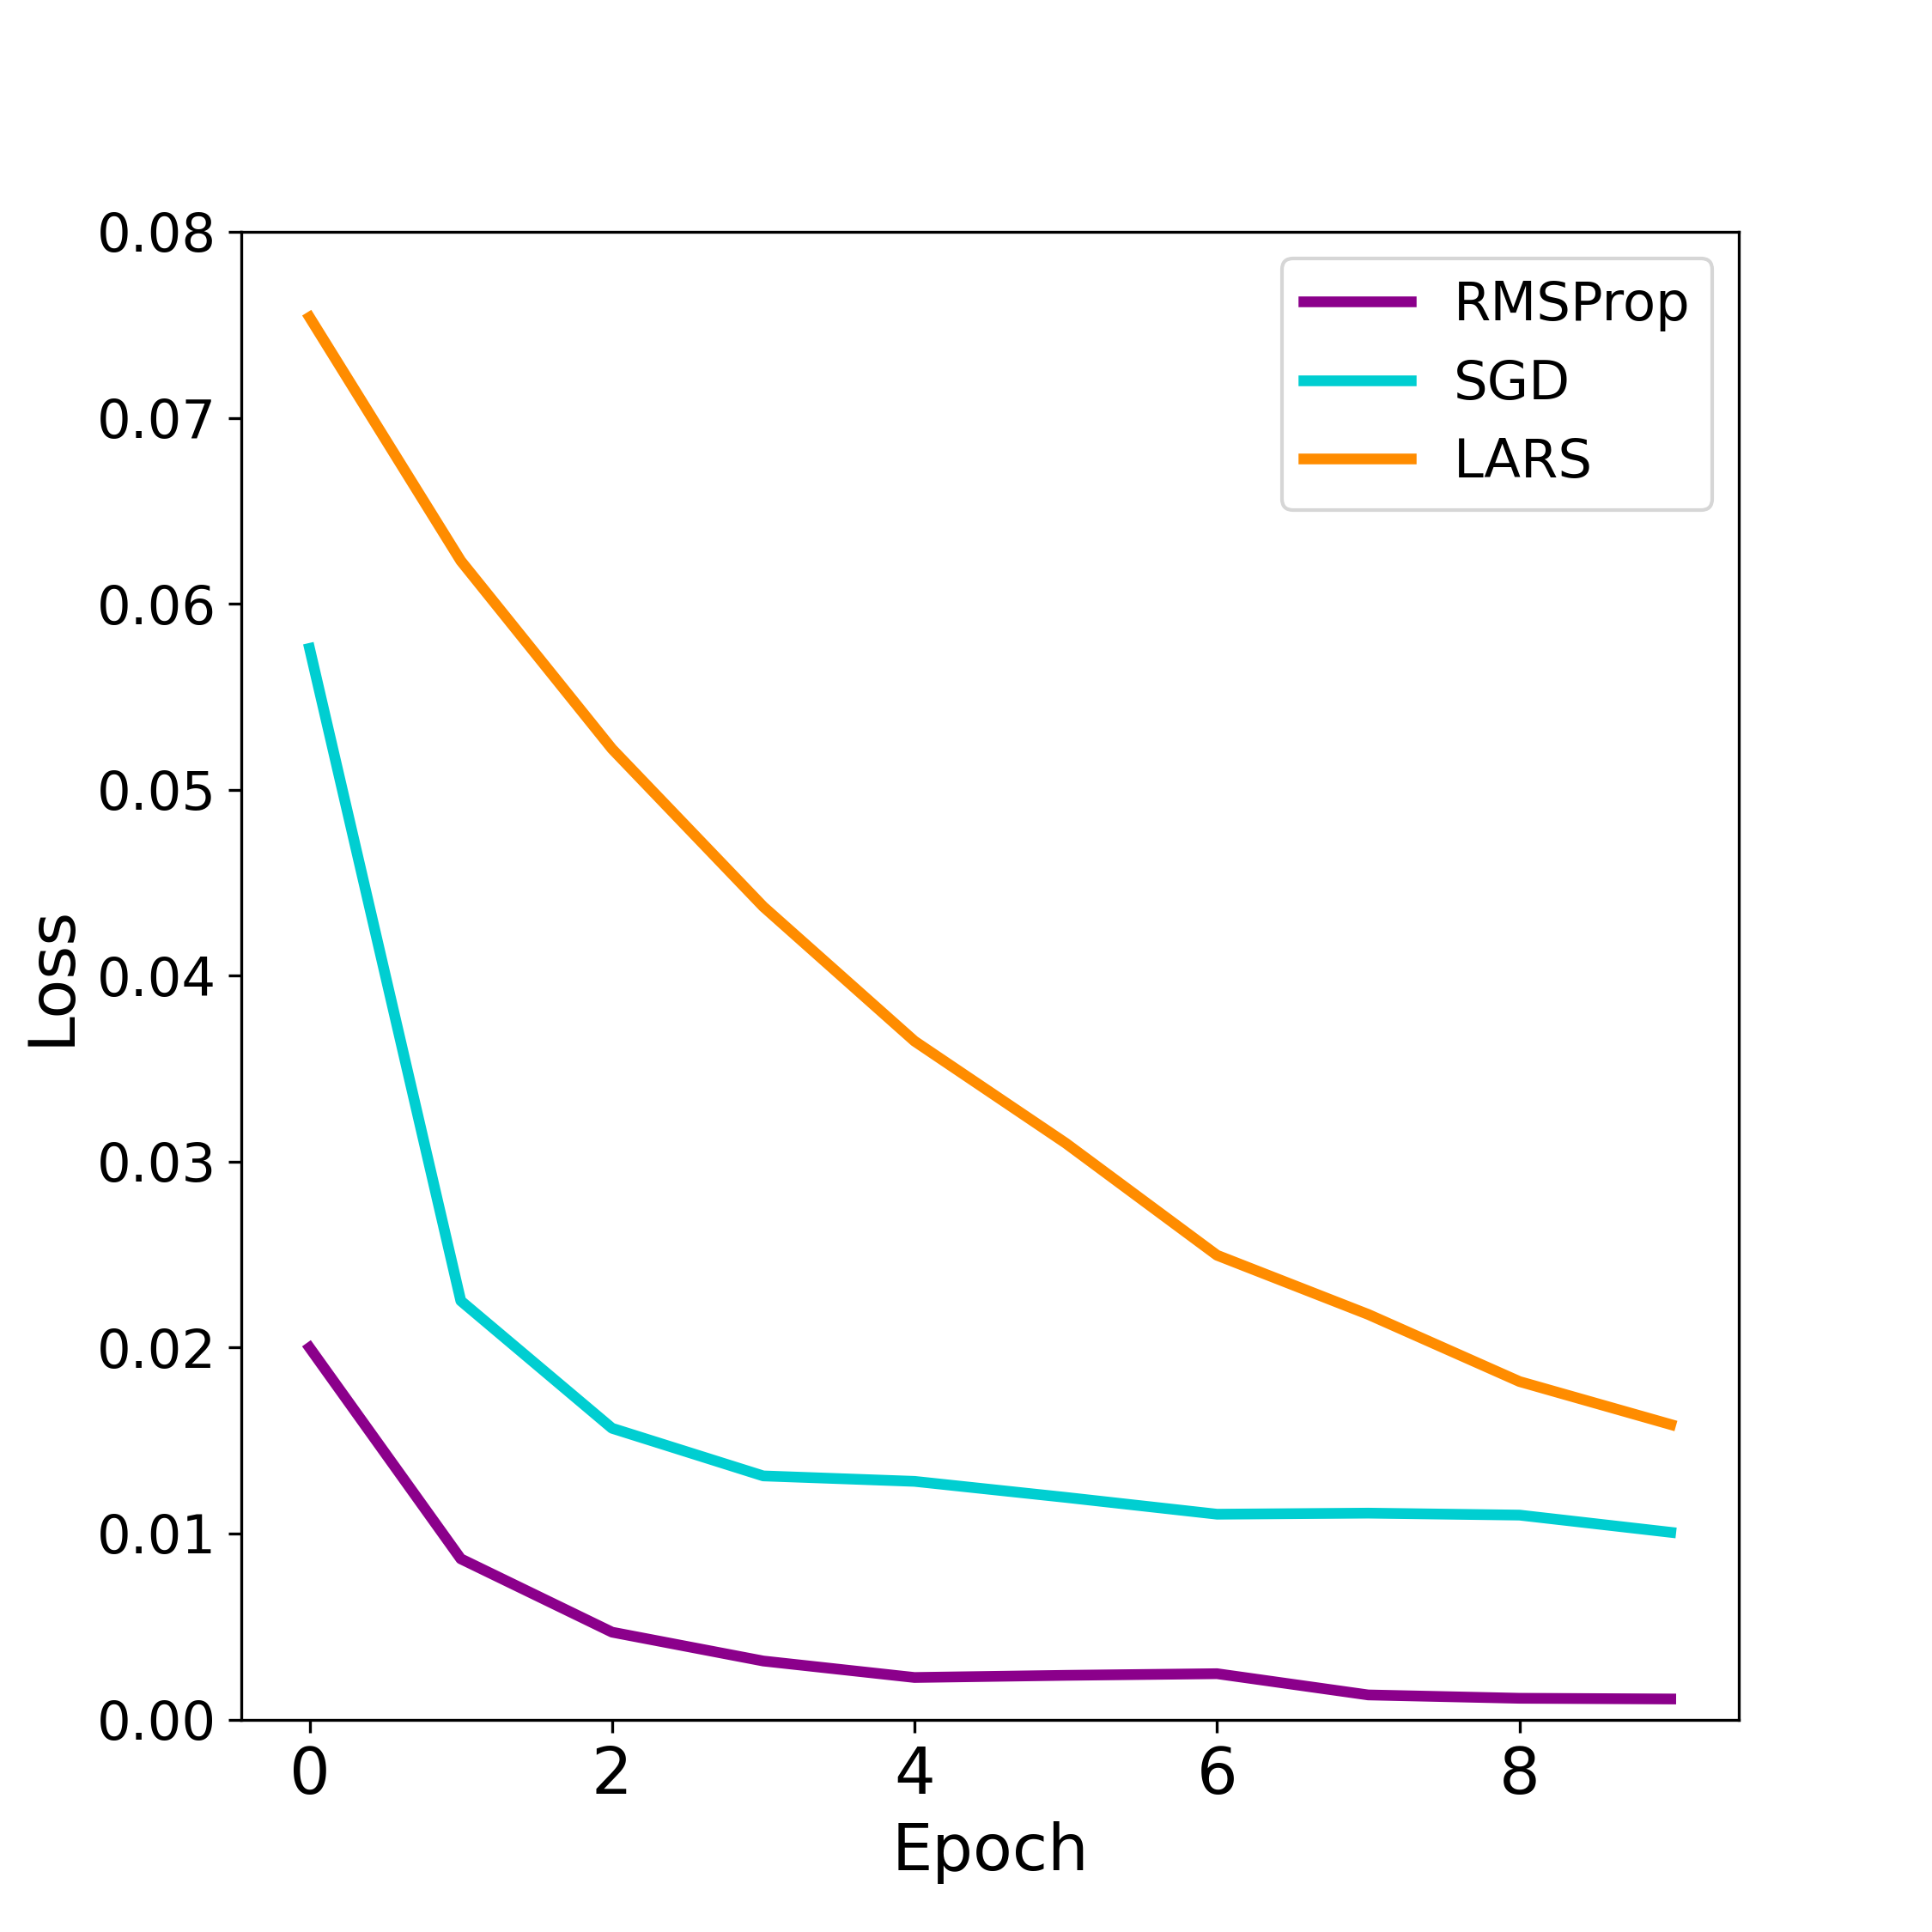
\includegraphics[width=0.45\textwidth]{Images/Pairwise_Train.png}\label{fig:infoOptTrain}}
  \subfloat[Loss on the validation set]{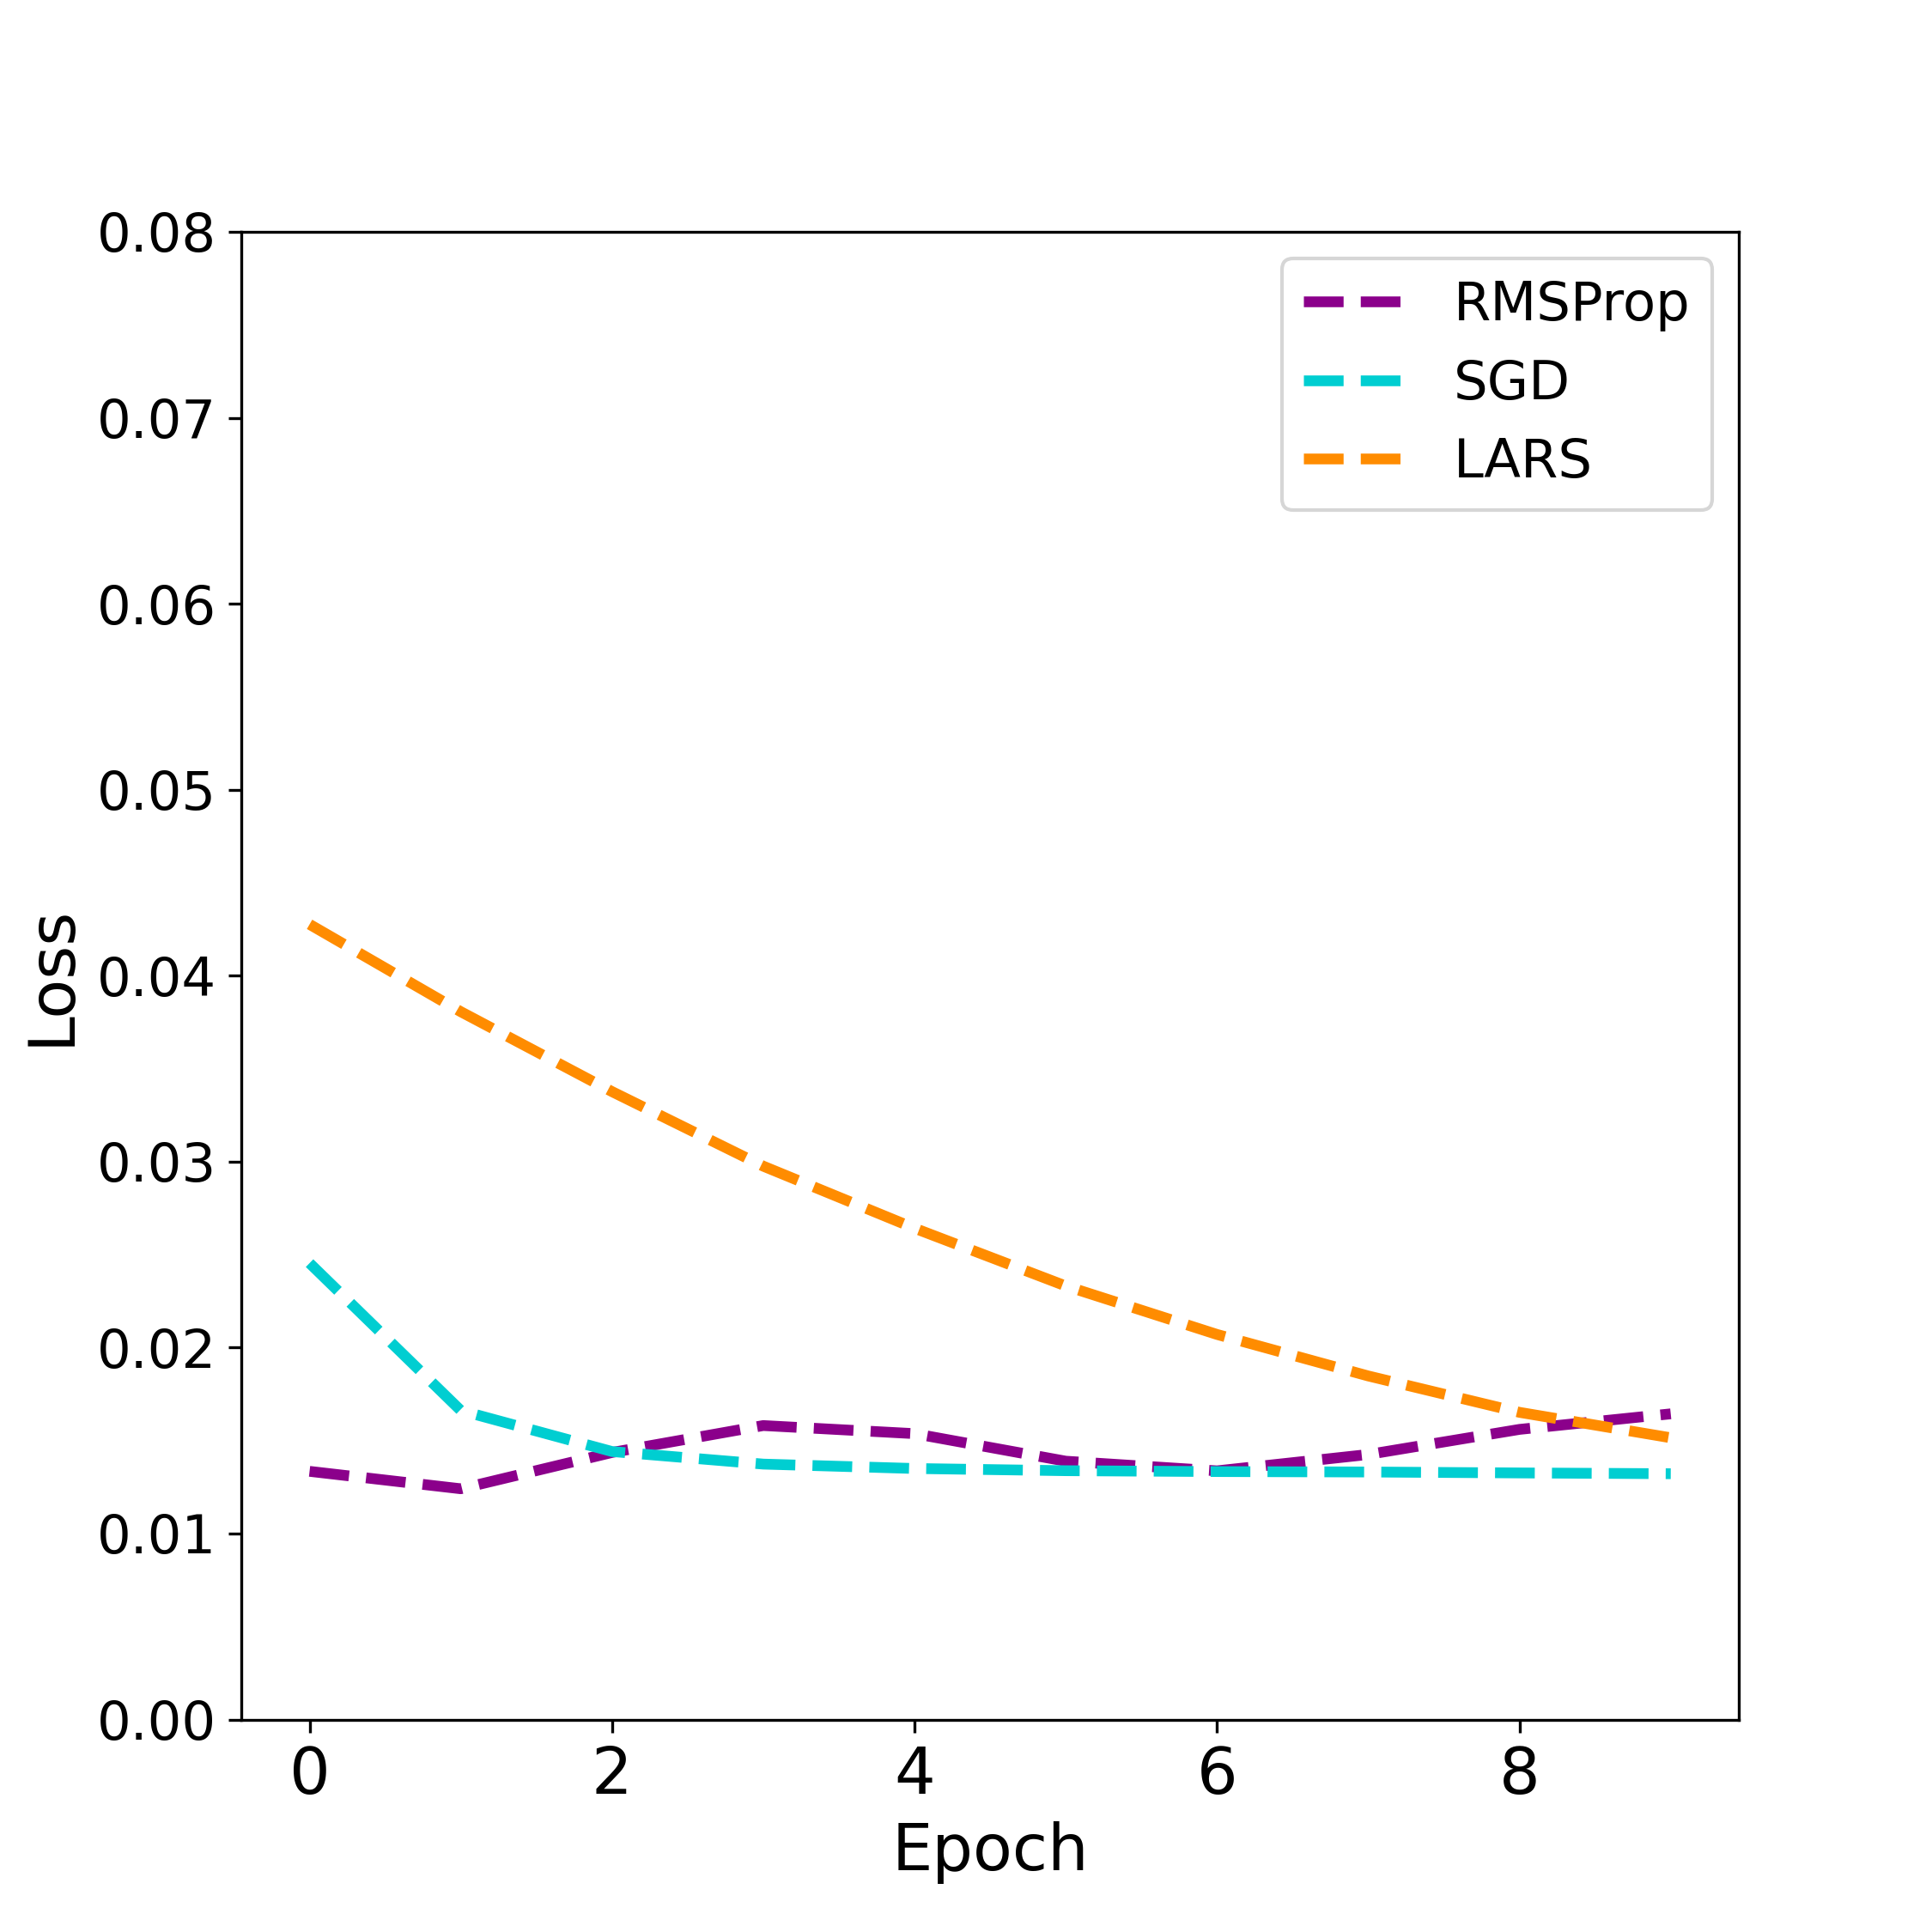
\includegraphics[width=0.45\textwidth]{Images/Pairwise_Validation.png}
  \label{fig:infoOptVal}}
  \caption{InfoNCE loss for different optimizers.}
  \label{fig:infoOpt}
\end{figure*}



\newpage
 
\newpage
\section{Example content}
The first line of the file must be
\begin{quote}
\begin{verbatim}
\documentclass[11pt]{article}
\end{verbatim}
\end{quote}

To load the style file in the review version:
\begin{quote}
\begin{verbatim}
\usepackage[review]{acl}
\end{verbatim}
\end{quote}
For the final version, omit the \verb|review| option:
\begin{quote}
\begin{verbatim}
\usepackage{acl}
\end{verbatim}
\end{quote}

To use Times Roman, put the following in the preamble:
\begin{quote}
\begin{verbatim}
\usepackage{times}
\end{verbatim}
\end{quote}
(Alternatives like txfonts or newtx are also acceptable.)

Please see the \LaTeX{} source of this document for comments on other packages that may be useful.

Set the title and author using \verb|\title| and \verb|\author|. Within the author list, format multiple authors using \verb|\and| and \verb|\And| and \verb|\AND|; please see the \LaTeX{} source for examples.

By default, the box containing the title and author names is set to the minimum of 5 cm. If you need more space, include the following in the preamble:
\begin{quote}
\begin{verbatim}
\setlength\titlebox{<dim>}
\end{verbatim}
\end{quote}
where \verb|<dim>| is replaced with a length. Do not set this length smaller than 5 cm.

\section{Document Body}

\subsection{Footnotes}

Footnotes are inserted with the \verb|\footnote| command.\footnote{This is a footnote.}

\subsection{Tables and figures}

See Table~\ref{tab:accents} for an example of a table and its caption.
\textbf{Do not override the default caption sizes.}

\begin{table}
\centering
\begin{tabular}{lc}
\hline
\textbf{Command} & \textbf{Output}\\
\hline
\verb|{\"a}| & {\"a} \\
\verb|{\^e}| & {\^e} \\
\verb|{\`i}| & {\`i} \\ 
\verb|{\.I}| & {\.I} \\ 
\verb|{\o}| & {\o} \\
\verb|{\'u}| & {\'u}  \\ 
\verb|{\aa}| & {\aa}  \\\hline
\end{tabular}
\begin{tabular}{lc}
\hline
\textbf{Command} & \textbf{Output}\\
\hline
\verb|{\c c}| & {\c c} \\ 
\verb|{\u g}| & {\u g} \\ 
\verb|{\l}| & {\l} \\ 
\verb|{\~n}| & {\~n} \\ 
\verb|{\H o}| & {\H o} \\ 
\verb|{\v r}| & {\v r} \\ 
\verb|{\ss}| & {\ss} \\
\hline
\end{tabular}
\caption{Example commands for accented characters, to be used in, \emph{e.g.}, Bib\TeX{} entries.}
\label{tab:accents}
\end{table}

\subsection{Hyperlinks}

Users of older versions of \LaTeX{} may encounter the following error during compilation: 
\begin{quote}
\tt\verb|\pdfendlink| ended up in different nesting level than \verb|\pdfstartlink|.
\end{quote}
This happens when pdf\LaTeX{} is used and a citation splits across a page boundary. The best way to fix this is to upgrade \LaTeX{} to 2018-12-01 or later.

\subsection{Citations}

\begin{table*}
\centering
\begin{tabular}{lll}
\hline
\textbf{Output} & \textbf{natbib command} & \textbf{Old ACL-style command}\\
\hline
\citep{Gusfield:97} & \verb|\citep| & \verb|\cite| \\
\citealp{Gusfield:97} & \verb|\citealp| & no equivalent \\
\citet{Gusfield:97} & \verb|\citet| & \verb|\newcite| \\
\citeyearpar{Gusfield:97} & \verb|\citeyearpar| & \verb|\shortcite| \\
\hline
\end{tabular}
\caption{\label{citation-guide}
Citation commands supported by the style file.
The style is based on the natbib package and supports all natbib citation commands.
It also supports commands defined in previous ACL style files for compatibility.
}
\end{table*}

Table~\ref{citation-guide} shows the syntax supported by the style files.
We encourage you to use the natbib styles.
You can use the command \verb|\citet| (cite in text) to get ``author (year)'' citations, like this citation to a paper by \citet{Gusfield:97}.
You can use the command \verb|\citep| (cite in parentheses) to get ``(author, year)'' citations \citep{Gusfield:97}.
You can use the command \verb|\citealp| (alternative cite without parentheses) to get ``author, year'' citations, which is useful for using citations within parentheses (e.g. \citealp{Gusfield:97}).

\subsection{References}

\nocite{Ando2005,borschinger-johnson-2011-particle,andrew2007scalable,rasooli-tetrault-2015,goodman-etal-2016-noise,harper-2014-learning}

The \LaTeX{} and Bib\TeX{} style files provided roughly follow the American Psychological Association format.
If your own bib file is named \texttt{custom.bib}, then placing the following before any appendices in your \LaTeX{} file will generate the references section for you:
\begin{quote}
\begin{verbatim}
\bibliographystyle{acl_natbib}
\bibliography{custom}
\end{verbatim}
\end{quote}

You can obtain the complete ACL Anthology as a Bib\TeX{} file from \url{https://aclweb.org/anthology/anthology.bib.gz}.
To include both the Anthology and your own .bib file, use the following instead of the above.
\begin{quote}
\begin{verbatim}
\bibliographystyle{acl_natbib}
\bibliography{anthology,custom}
\end{verbatim}
\end{quote}

Please see Section~\ref{sec:bibtex} for information on preparing Bib\TeX{} files.

\subsection{Appendices}

Use \verb|\appendix| before any appendix section to switch the section numbering over to letters. See Appendix~\ref{sec:appendix} for an example.

\section{Bib\TeX{} Files}
\label{sec:bibtex}

Unicode cannot be used in Bib\TeX{} entries, and some ways of typing special characters can disrupt Bib\TeX's alphabetization. The recommended way of typing special characters is shown in Table~\ref{tab:accents}.

Please ensure that Bib\TeX{} records contain DOIs or URLs when possible, and for all the ACL materials that you reference.
Use the \verb|doi| field for DOIs and the \verb|url| field for URLs.
If a Bib\TeX{} entry has a URL or DOI field, the paper title in the references section will appear as a hyperlink to the paper, using the hyperref \LaTeX{} package.

\section*{Acknowledgements}

This document has been adapted
by Steven Bethard, Ryan Cotterell and Rui Yan
from the instructions for earlier ACL and NAACL proceedings, including those for 
ACL 2019 by Douwe Kiela and Ivan Vuli\'{c},
NAACL 2019 by Stephanie Lukin and Alla Roskovskaya, 
ACL 2018 by Shay Cohen, Kevin Gimpel, and Wei Lu, 
NAACL 2018 by Margaret Mitchell and Stephanie Lukin,
Bib\TeX{} suggestions for (NA)ACL 2017/2018 from Jason Eisner,
ACL 2017 by Dan Gildea and Min-Yen Kan, 
NAACL 2017 by Margaret Mitchell, 
ACL 2012 by Maggie Li and Michael White, 
ACL 2010 by Jing-Shin Chang and Philipp Koehn, 
ACL 2008 by Johanna D. Moore, Simone Teufel, James Allan, and Sadaoki Furui, 
ACL 2005 by Hwee Tou Ng and Kemal Oflazer, 
ACL 2002 by Eugene Charniak and Dekang Lin, 
and earlier ACL and EACL formats written by several people, including
John Chen, Henry S. Thompson and Donald Walker.
Additional elements were taken from the formatting instructions of the \emph{International Joint Conference on Artificial Intelligence} and the \emph{Conference on Computer Vision and Pattern Recognition}.



\end{document}
